%!TEX root = thesis.tex
\chapter{Benchmarking results and analysis}
\label{ch:bmresults}

The encoding, decoding, and file size performance are presented first in this Chapter as these results can help explaining the results in other parts, but they are naturally factored within the benchmarks of the operations (see Section~\ref{sec:operations}) as well.
After this the time benchmarks of the remaining performance indicators (see Table~\ref{tab:indicators}) are shown in separate sections.
These Sections are subsequently divided per operation and by server implementation (with compression in advance or compression on the fly).
Lastly there is a conclusion including a plot where all operations are averaged.


The datasets (see Section~\ref{datasetdescription}) are divided in two classes: bigger (Singapore, TUDelft, New York, and Zürich) and small datasets (Delft, Den Haag, Rotterdam, and Montréal). 
I arbitrarily did this because showing the results per dataset makes it too complex, while the file size is the clearest divide between the datasets and also a factor that is expected to be significant for the performance.
In addition to that, for every dataset there is a variant from which the attributes are removed, with which it can be shown how the presence of attributes impacts compression.

Since the results are averaged by dataset group, box plots are presented.
These show some statistics as well on the variety of the datasets within a dataset group.
In the charts that show the performance of an operation on a compressed dataset, the baseline (uncompressed CityJSON) is shown with a dotted line.
The time multiplier on the x-axis shows how much time it took to complete the specific task as compared to the baseline---a time multiplier of 0.5 means that it took half the time of doing the same thing with uncompressed CityJSON, and a time multiplier of 2 means that it took twice as long.
The scales of the plots are not always fixed, which means that the four plots (large, large without attributes, small, and small without attributes) within one figure can have different scales.
This requires extra attention when interpreting the results, but it is necessary to make them readable when the time multipliers between the two plots are very different.

Besides these plots, for all operations a table is added that shows the median performance of every compression type per dataset type.
It is sorted ascendingly so that it can easily be seen which compression types are the best for the corresponding operation.


The conclusion (Section~\ref{bmconclusion}) gives an overview of the results, indicating the advantages and disadvantages of every compression type.
It includes two plots that show an overview of the performance of the compression types (Figures~\ref{fig:performanceoverview} and~\ref{fig:performanceoverviewotf}).
Again per dataset group, but with all operations averaged.
Through this it can more easily be noticed how different compression types compare when the wanted operation is unknown.
Thus answering the question: "when you want to compress a dataset of this size and use it for any kind of purpose, which compression type would be advisable?".

Tables of the full results that are used to create the charts of the operations are found in Appendix~\ref{ap:raw}.
For some combinations of use cases and compression types there were errors in the benchmarking.
These are shown in those tables with \texttt{NA} and it results in missing compression types or strange looking boxplots in the charts.


\newpage
\section{Encoding performance}
\label{sec:encodingperformance}

\begin{figure}[h!]
    %\hspace*{-2.3cm}  
    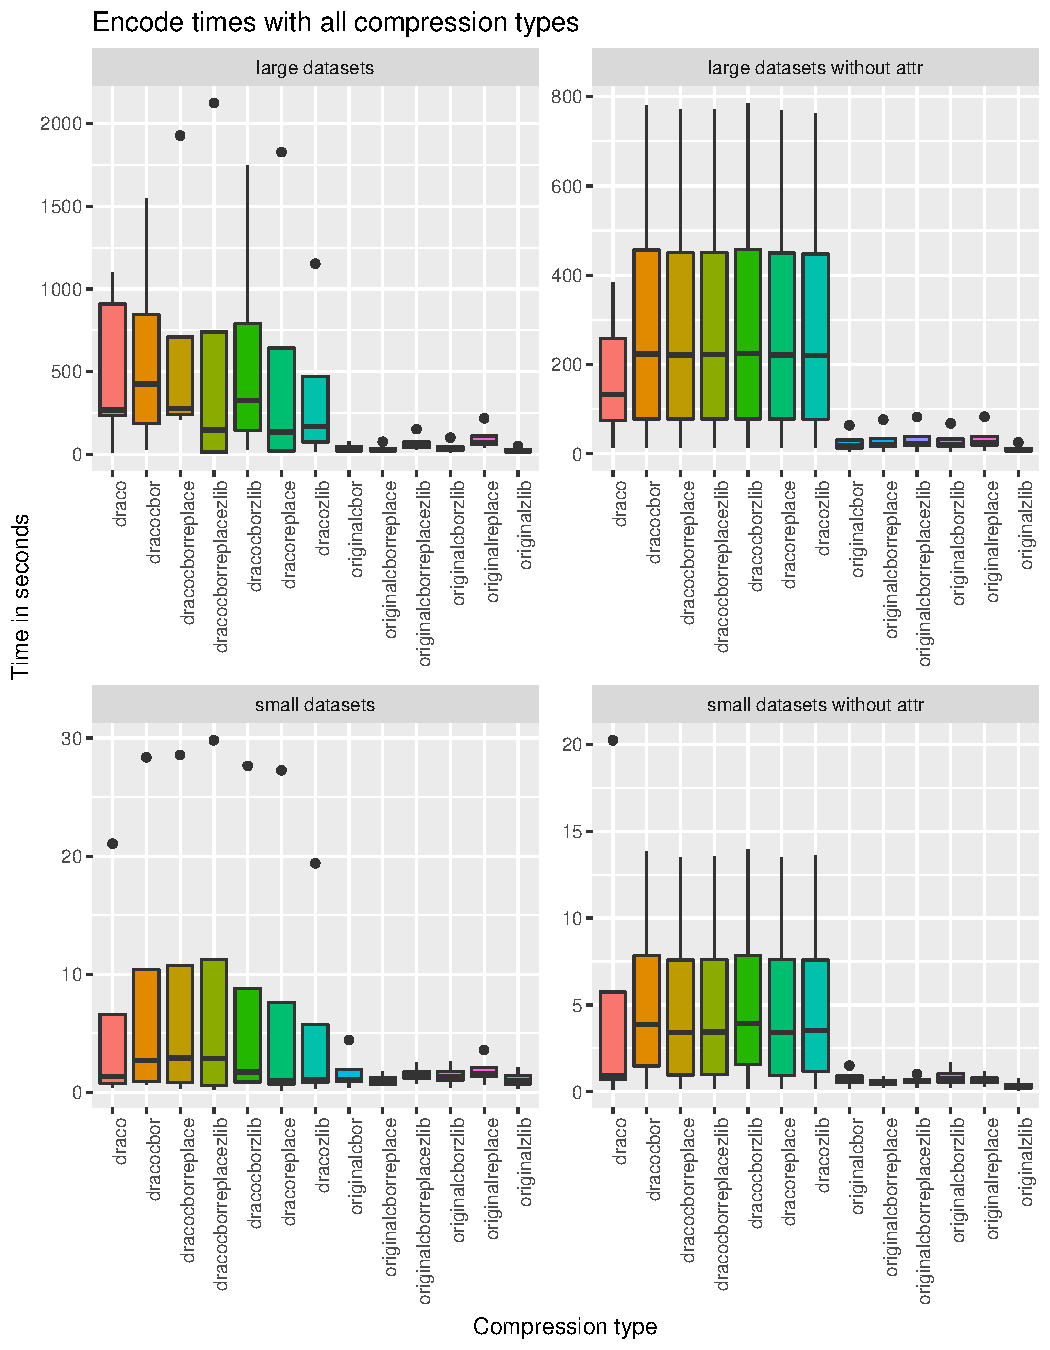
\includegraphics[scale=0.88]{figs/benchmark/overview/encodingtimes.pdf}
    \caption{Boxplots of the encoding time performance of different compression types.}
    \label{fig:encodingperformance}
\end{figure}


The encoding times shown here only apply to the preparation of datasets in Python (which is linked to C++ for Draco compression).
Therefore they are not an influence on the other performance results.
After editing datasets they also need to be encoded, but this is done in the client and not in the server in the case of compression in advance.
Encoding times in the client are incorporated in the editing benchmark results for that use case.

For datasets with attributes, compression types that include Draco always take considerably longer to encode, which is true for both bigger and small datasets.
That the impact is this large is likely because of a CityJSON dataset having to be converted to OBJ first before it can be encoded by Draco.
For large datasets, Draco compression itself already takes four minutes.
It could become a large share of the execution time of the preparation of datasets.
For small datasets this is not a problem because it is still fast in absolute terms, but it is still more expensive.

Draco-cbor on average takes longest for bigger datasets.
Combining it in draco-cbor-replace-zlib it is faster.
Possibly this is because \ac{cbor} can encode the keys and values of a dataset faster in this structure, where all strings are contained in one array and encoded in zlib which results in a binary value.
For small datasets these two compression types have similar performance, so the difference in JSON-structure (which is parsed into CBOR) is only noticed with a large dataset.
Draco-cbor-replace-zlib is the fastest of the Draco ones together with draco-replace.

I had expected that the replace method would be expensive, but there is no clear pattern in it.
Draco-replace is faster than the other Draco types for bigger datasets, but original-replace is the slowest one without Draco.
The other types that use replace but also are in CBOR are encoded faster, despite having more steps in the compression.
It could possibly explained by CBOR being written to a file faster than JSON, or it is just simply written faster due to its size being smaller.

Original-zlib is however the fastest on the bigger datasets.
Zlib thus seems to be the fastest compression technique to use on bigger datasets, but with smaller ones it is not significantly faster than others.
Based on both plots, original-cbor, original-cbor-replace, or original-zlib would be the best choices if the encoding time is important.

As for the datasets from which the attributes are stripped, the results are not very much different.
For both the large and the small datasets the encoding time is lower, which is to be expected since there is less data to compress.
With the large datasets you also see that the median times for the compression types seem more uniform, which is because the geometry compression is now relatively more important, and this is generally divided into Draco compression versus (more or less) retaining the structure of the original geometries (but they are most of the time still compressed by zlib or CBOR, see Section~\ref{sec:compressiondecompression}).






\newpage
\section{Decoding performance}
\label{sec:decodingperformance}

\begin{figure}[h!]
    %\hspace*{-2.3cm}  
    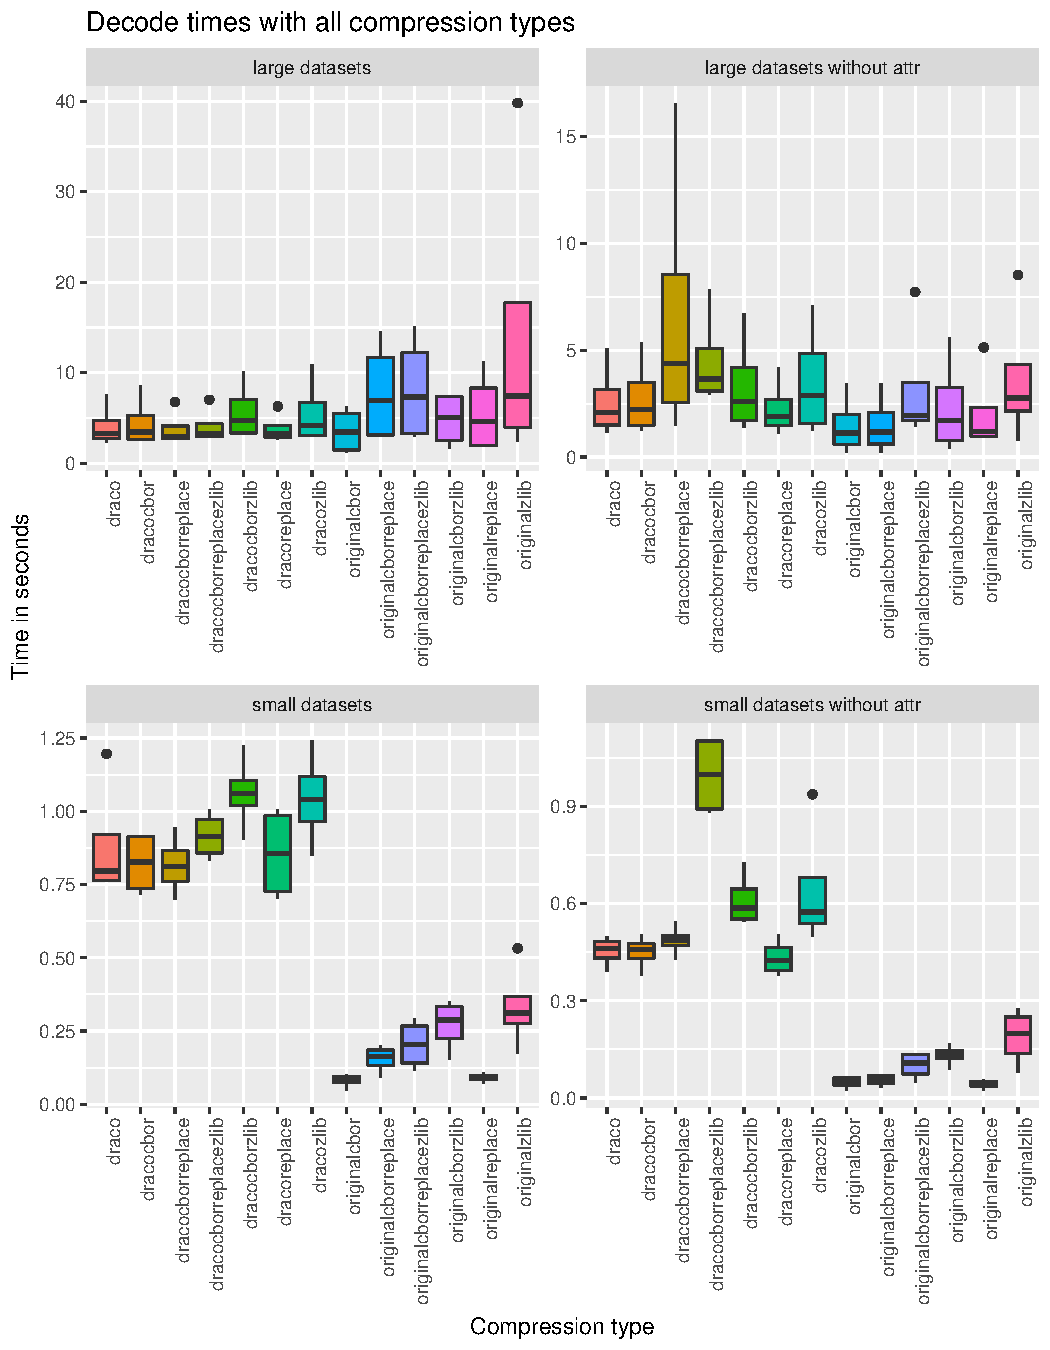
\includegraphics[scale=0.88]{figs/benchmark/overview/decodingtimes.pdf}
    \caption{Boxplots of the decoding time performance of different compression types.}
    \label{fig:decodingtimes}
\end{figure}


The decoding times are shown with a normal scale as the results do not have a large spread as there was with the encoding performance.
These statistics should be a significant explaining factor throughout the results chapter as it is a main property that explains the difference in performance between varying compression types.

While encoding Draco took a comparatively long time, it is generally decoded quicker with the bigger datasets (with attributes) than the other compression types.
This is not the case for the small datasets, suggesting that the larger a dataset is, the more suitable it is to use Draco.

Original-cbor on the other hand has a low mean decoding time as well, for both dataset types.
Combining CBOR in any way with replace will decrease the performance, probably because it is expensive to traverse all keys and values and replace them.

Original-zlib takes long to decode, contrasting its encoding results.
Its outlier on the left plot is the Zürich dataset, which took a considerably longer time than decoding the same dataset compressed in another way.
The extent of the corresponding box plot also indicates that the larger a dataset is, the longer it takes to decode it as compared to the other compression types. 
This can potentially pose to be a disadvantage of original-zlib.

The datasets without attributes again show faster performance since there is less data to decode.
Because the replace method has (almost) no attributes to decode, it now adds less time to the decompression, although it is probably also not useful to use it when compared to original CityJSON.
However, draco-cbor-replace (large datasets without attributes) and draco-cbor-replace-zlib (small datasets without attributes) do have notably higher decoding times, but I do not see plausible explanations for this.



\newpage
\section{File size}
\label{sec:filesizeperformance}

\begin{figure}[h!]
    %\hspace*{-2.3cm}  
    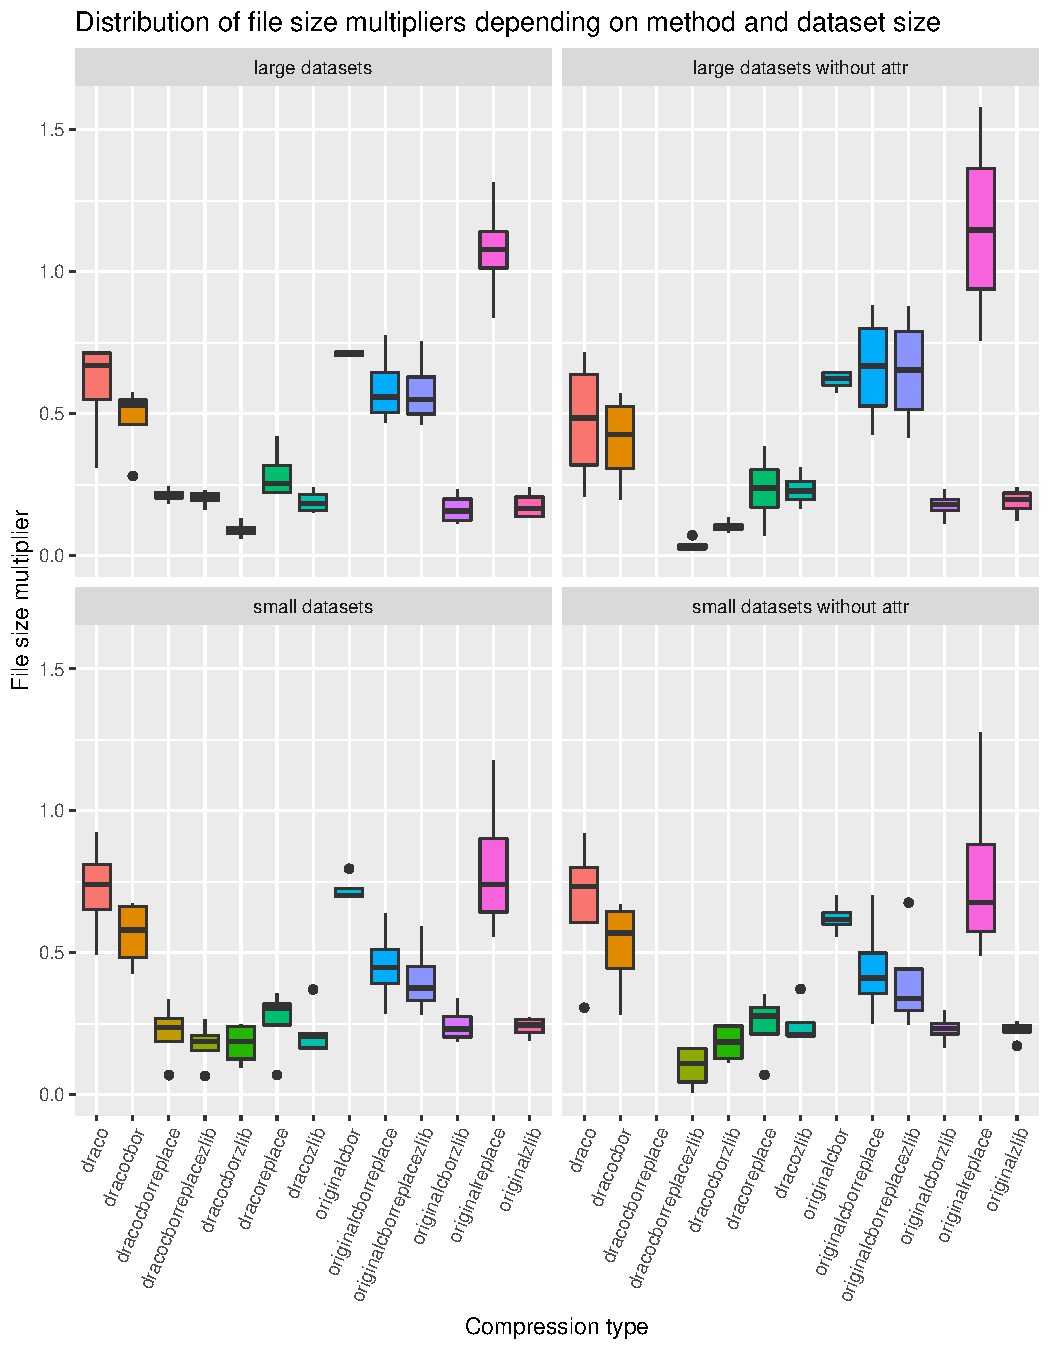
\includegraphics[scale=0.88]{figs/benchmark/overview/filesizemultipliers.pdf}
    \caption{Boxplots of file size multipliers indicating to which extent compression types compress the data.}
    \label{fig:filesizeperformance}
\end{figure}

The file size multipliers are similar between the bigger and small datasets, and datasets with or without attributes.
The latter observation indicates that the compression of actual city object attributes does not contribute as much to compression as a whole, and that the compression of geometries, the JSON structure (CBOR), and general purpose compression (zlib) are more beneficial, with the latter two also naturally compressing the attributes of city objects when they are used.
It is again shown that compressing geometry with Draco is mostly suitable for bigger datasets.
These datasets have a lower file size multiplier than the small datasets compressed with Draco.

Original-replace is the only compression type that in some cases makes a file larger than the original.
The array of attributes is then larger than the removed redundancy.
The replace method in general does not yield very favourable results, even when the array of attributes is encoded.

Combining CBOR and zlib or using zlib only gives the smallest file sizes when compressing bigger datasets, for both Draco compression types and the ones with original geometry.
This trend is seen for the small datasets as well.
So compression types with zlib are both encoded quickly (Section~\ref{sec:encodingperformance}) and yield small files.
On the other hand zlib takes long to decode as shown in Section~\ref{sec:decodingperformance}.
Further performance benchmarks will thus demonstrate whether or not the decreased file sized outweighs the increased decoding time.








\newpage
\section{Visualisation}
\label{bmvisualisation}

\subsection{Compression in advance}

\begin{figure}[h!]
    %\hspace*{-2.3cm}  
    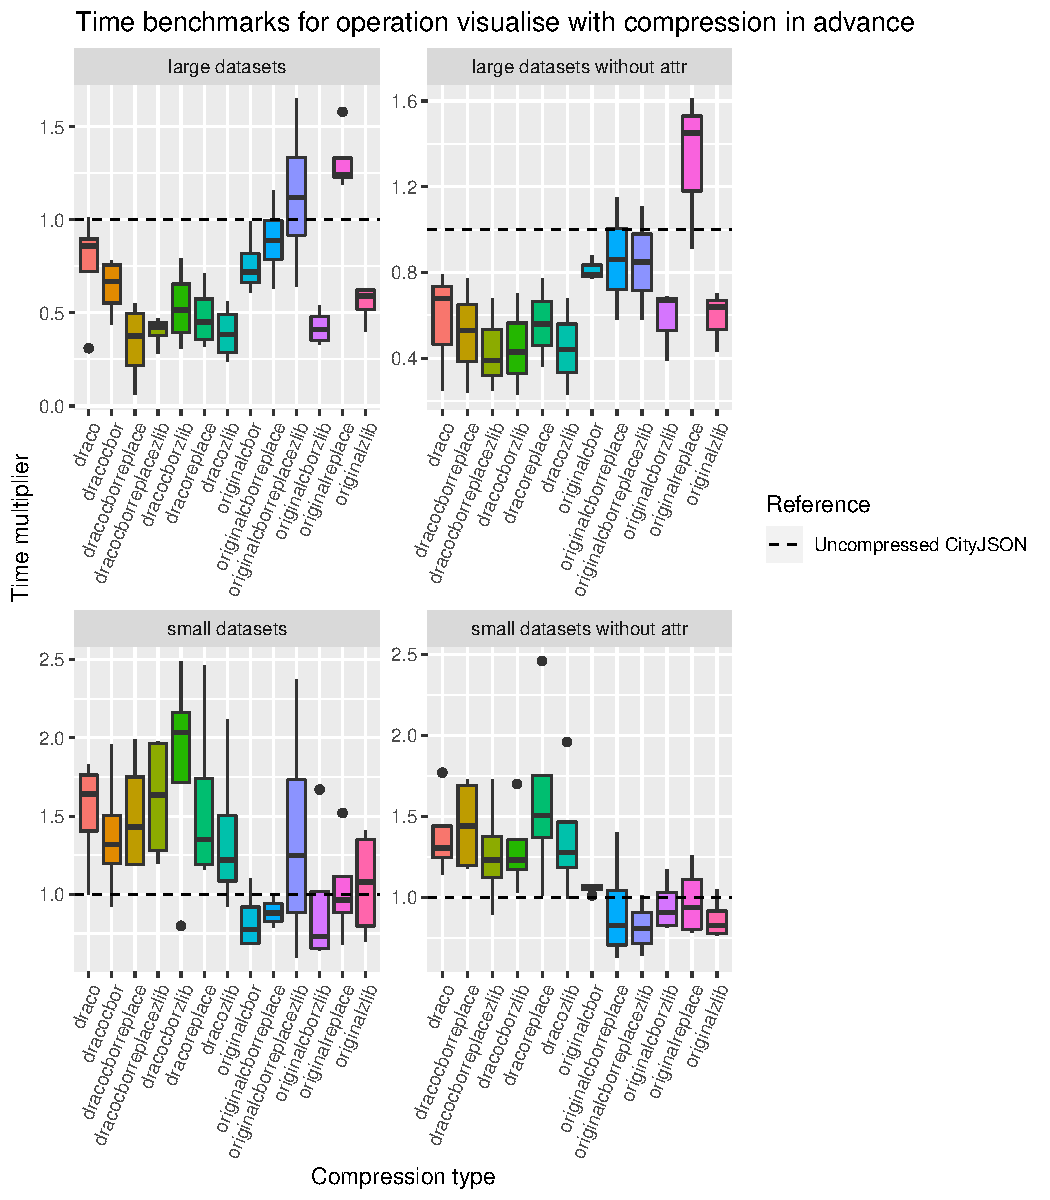
\includegraphics[scale=0.88]{figs/benchmark/individual/visualise.pdf}
    \caption{Boxplots of time performance of (in advance) compressed datasets on visualisation compared to uncompressed CityJSON.}
    \label{fig:sdvis}
\end{figure}


Visualising compressed small datasets often yields a performance that is worse than the baseline, but this is especially the case when using Draco.
It is not worth using it for small data, which can be explained by the overhead of Draco compression contributing a relatively large part in performance time.
This is the same for small datasets that do not contain attributes.
On the other hand, original-cbor and original-cbor-zlib have a good median performance. Orginal-cbor-replace is an acceptable option as well.
When not having to compress attributes, all compression types with original geometries retained do pretty well, except for orginal-cbor that suddenly has its median above the baseline, which is unexpected as this is not the case when attributes are included.
It could be an abnormality in the benchmarking.

But for large datasets it is even more beneficial to use compression in general.
With this use case it turns out that it can be worth it to use Draco if performance time is most important.
But some compression types without it also do well, especially original-cbor-zlib and original-zlib.
Even when attributes are not included, additional compression besides Draco proves to be useful as using Draco only comparatively performs worst amongst the Draco compression types.

Compression can improve the visualisation time of CityJSON datasets to 37\%, 39\%, 73\%, or 80\% (when respectively using large datasets, large datasets without attributes, small datasets, and small datasets without attributes) of the time that it takes to perform the same operation with uncompressed CityJSON, in the case of compressing the dataset in advance.


  \begin{table}[!h]
    \begin{minipage}{.5\linewidth}
      \caption{
Median performance with visualise on large datasets, compression in advance}
\centering

\begin{tabular}{|l|r|}
\hline
Compression type & median\\
\hline
dracocborreplace & 0.375\\
\hline
dracozlib & 0.385\\
\hline
originalcborzlib & 0.410\\
\hline
dracocborreplacezlib & 0.425\\
\hline
dracoreplace & 0.450\\
\hline
dracocborzlib & 0.515\\
\hline
originalzlib & 0.590\\
\hline
dracocbor & 0.670\\
\hline
originalcbor & 0.720\\
\hline
draco & 0.860\\
\hline
originalcborreplace & 0.890\\
\hline
originalcborreplacezlib & 1.120\\
\hline
originalreplace & 1.245\\
\hline
\end{tabular}
\end{minipage}%
    \begin{minipage}{.5\linewidth}
      \centering
        \caption{
Median performance with visualise on large datasets without attributes, compression in advance}

\begin{tabular}{|l|r|}
\hline
Compression type & median\\
\hline
dracocborreplacezlib & 0.39\\
\hline
dracocborzlib & 0.43\\
\hline
dracozlib & 0.44\\
\hline
dracocborreplace & 0.53\\
\hline
dracoreplace & 0.56\\
\hline
originalzlib & 0.64\\
\hline
originalcborzlib & 0.67\\
\hline
draco & 0.68\\
\hline
originalcbor & 0.79\\
\hline
originalcborreplacezlib & 0.85\\
\hline
originalcborreplace & 0.86\\
\hline
originalreplace & 1.45\\
\hline
\end{tabular}
\end{minipage} 
\end{table}
\begin{table}[!h]
    \begin{minipage}{.5\linewidth}
      \caption{
Median performance with visualise on small datasets, compression in advance}
\centering

\begin{tabular}{|l|r|}
\hline
Compression type & median\\
\hline
originalcborzlib & 0.730\\
\hline
originalcbor & 0.775\\
\hline
originalcborreplace & 0.880\\
\hline
originalreplace & 0.965\\
\hline
originalzlib & 1.080\\
\hline
dracozlib & 1.220\\
\hline
originalcborreplacezlib & 1.250\\
\hline
dracocbor & 1.320\\
\hline
dracoreplace & 1.350\\
\hline
dracocborreplace & 1.430\\
\hline
dracocborreplacezlib & 1.635\\
\hline
draco & 1.640\\
\hline
dracocborzlib & 2.035\\
\hline
\end{tabular}
\end{minipage}%
    \begin{minipage}{.5\linewidth}
      \centering
        \caption{
Median performance with visualise on small datasets without attributes, compression in advance}

\begin{tabular}{|l|r|}
\hline
Compression type & median\\
\hline
originalcborreplacezlib & 0.805\\
\hline
originalcborreplace & 0.825\\
\hline
originalzlib & 0.825\\
\hline
originalcborzlib & 0.905\\
\hline
originalreplace & 0.935\\
\hline
originalcbor & 1.065\\
\hline
dracocborreplacezlib & 1.230\\
\hline
dracocborzlib & 1.230\\
\hline
dracozlib & 1.275\\
\hline
draco & 1.305\\
\hline
dracocborreplace & 1.440\\
\hline
dracoreplace & 1.505\\
\hline
\end{tabular}
\end{minipage} 
\end{table}

\clearpage

\subsection{Compression on the fly}

\begin{figure}[h!]
    %\hspace*{-2.3cm}  
    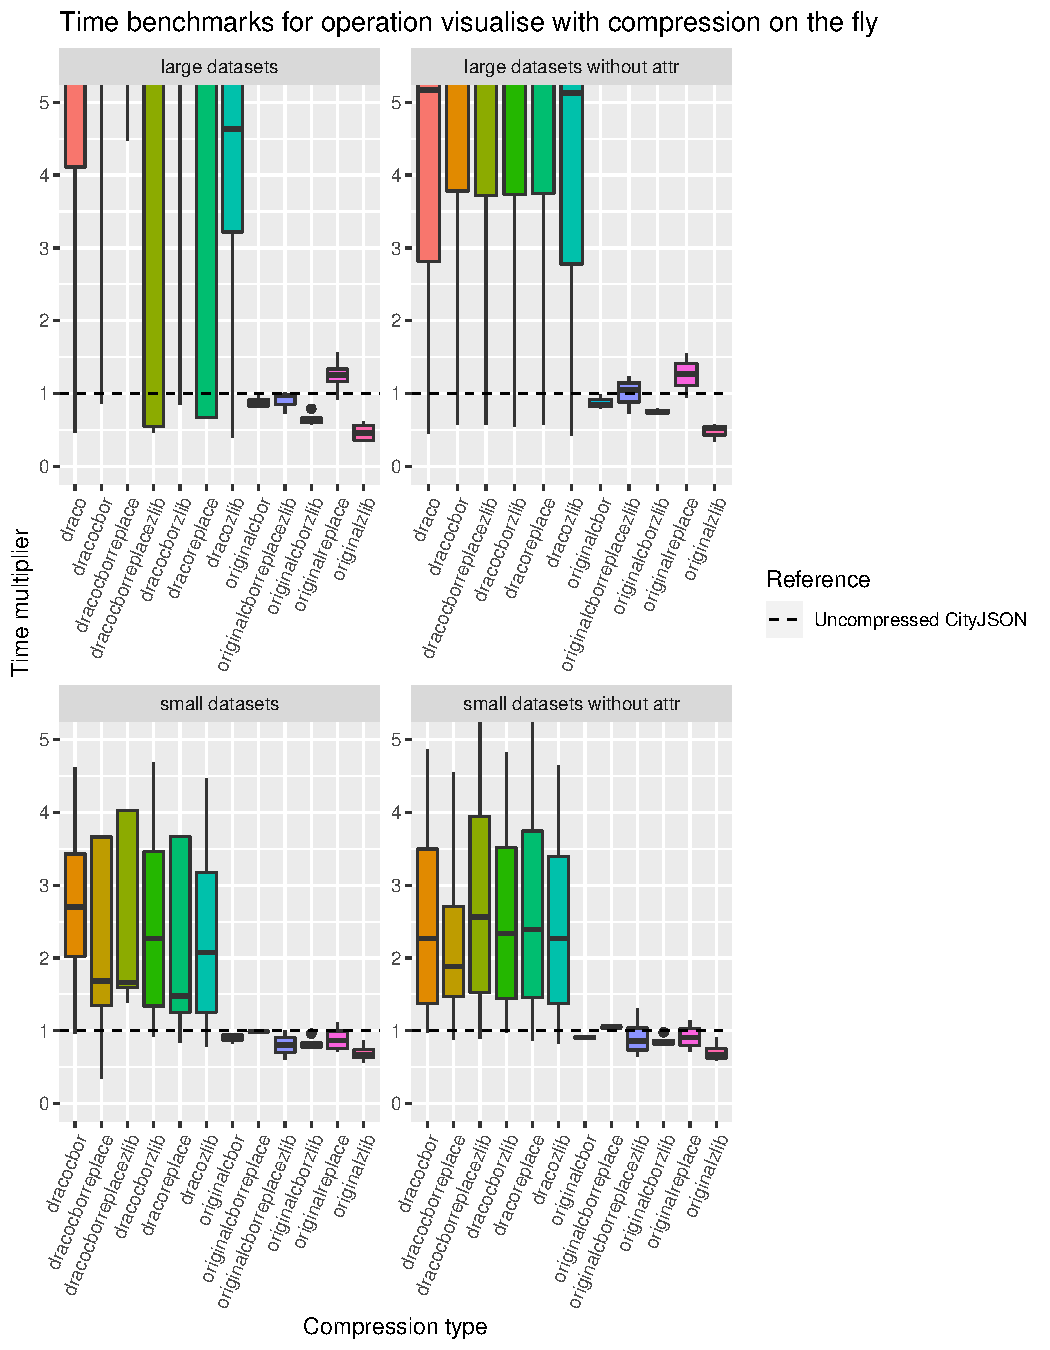
\includegraphics[scale=0.88]{figs/benchmark/individualotf/visualise.pdf}
    \caption{Boxplots of time performance of (on the fly) compressed datasets on visualisation compared to uncompressed CityJSON.}
    \label{figotf:sdvis}
\end{figure}

When compressing data after a request for the visualisation of a full dataset is made, the performance is slower since now the compression time of the compression type is of influence on the results.
This means that none of the compression types using Draco are suitable for use, since it takes relatively long to compress (which is also influenced by having to convert the geometries to OBJ first, see Section~\ref{sec:dracocompressiontypes}).
They are all way above the performance baseline.
The y-scale of the graphs is limited for this reason.

Compression types that do not use Draco are generally beneficial.
Original-cbor, original-cbor-zlib, and original-zlib are best to use, without distinguishment between dataset type.
The median performance gain is however slightly larger for large datasets.

On the fly compression can improve the visualisation time of CityJSON datasets to 45\%, 52\%, 67\%, or 67\% (when respectively using large datasets, large datasets without attributes, small datasets, and small datasets without attributes) of the time that it takes to perform the same operation with uncompressed CityJSON, in the case of compressing the dataset on the fly.



\begin{table}[!h]
    \begin{minipage}{.5\linewidth}
      \caption{
Median performance with visualise on large datasets, compression on the fly}
\centering

\begin{tabular}{|l|r|}
\hline
Compression type & median\\
\hline
originalzlib & 0.455\\
\hline
originalcborzlib & 0.615\\
\hline
originalcbor & 0.860\\
\hline
originalcborreplacezlib & 0.970\\
\hline
originalreplace & 1.255\\
\hline
dracozlib & 4.635\\
\hline
draco & 5.580\\
\hline
dracoreplace & 6.015\\
\hline
dracocborreplacezlib & 6.460\\
\hline
dracocborreplace & 8.670\\
\hline
dracocborzlib & 8.705\\
\hline
dracocbor & 11.465\\
\hline
\end{tabular}
\end{minipage}%
    \begin{minipage}{.5\linewidth}
      \centering
        \caption{
Median performance with visualise on large datasets without attributes, compression on the fly}

\begin{tabular}{|l|r|}
\hline
Compression type & median\\
\hline
originalzlib & 0.52\\
\hline
originalcborzlib & 0.74\\
\hline
originalcbor & 0.85\\
\hline
originalcborreplacezlib & 1.05\\
\hline
originalreplace & 1.27\\
\hline
dracozlib & 5.13\\
\hline
draco & 5.17\\
\hline
dracocborreplacezlib & 6.86\\
\hline
dracocborzlib & 6.92\\
\hline
dracoreplace & 6.93\\
\hline
dracocbor & 6.99\\
\hline
\end{tabular}
\end{minipage} 
\end{table}
\begin{table}[!h]
    \begin{minipage}{.5\linewidth}
      \caption{
Median performance with visualise on small datasets, compression on the fly}
\centering

\begin{tabular}{|l|r|}
\hline
Compression type & median\\
\hline
originalzlib & 0.675\\
\hline
originalcborzlib & 0.790\\
\hline
originalcborreplacezlib & 0.805\\
\hline
originalreplace & 0.865\\
\hline
originalcbor & 0.915\\
\hline
originalcborreplace & 0.990\\
\hline
dracoreplace & 1.475\\
\hline
dracocborreplacezlib & 1.665\\
\hline
dracocborreplace & 1.685\\
\hline
dracozlib & 2.075\\
\hline
dracocborzlib & 2.265\\
\hline
dracocbor & 2.700\\
\hline
\end{tabular}
\end{minipage}%
    \begin{minipage}{.5\linewidth}
      \centering
        \caption{
Median performance with visualise on small datasets without attributes, compression on the fly}

\begin{tabular}{|l|r|}
\hline
Compression type & median\\
\hline
originalzlib & 0.670\\
\hline
originalcborzlib & 0.830\\
\hline
originalcborreplacezlib & 0.860\\
\hline
originalreplace & 0.910\\
\hline
originalcbor & 0.910\\
\hline
originalcborreplace & 1.050\\
\hline
dracocborreplace & 1.880\\
\hline
dracocbor & 2.270\\
\hline
dracozlib & 2.270\\
\hline
dracocborzlib & 2.340\\
\hline
dracoreplace & 2.390\\
\hline
dracocborreplacezlib & 2.565\\
\hline
\end{tabular}
\end{minipage} 
\end{table}




\section{Querying}
\label{bmquerying}

\subsection{Querying one feature}

\subsubsection{Compression in advance}

\begin{figure}[h!]
    %\hspace*{-2.3cm}  
    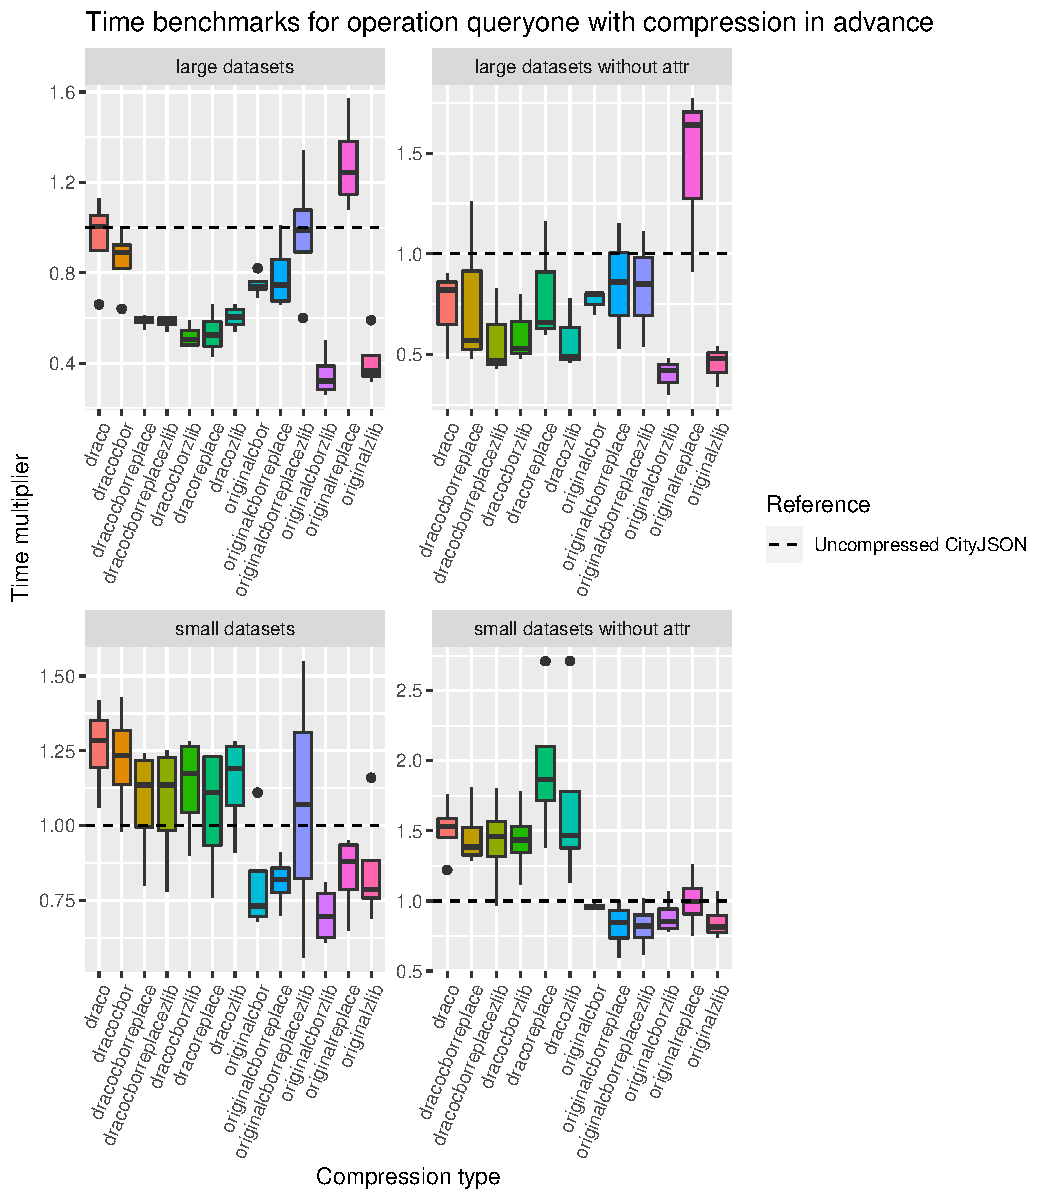
\includegraphics[scale=0.92]{figs/benchmark/individual/queryone.pdf}
    \caption{Boxplots of time performance of (in advance) compressed datasets on querying one feature compared to uncompressed CityJSON.}
    \label{fig:sdvis}
\end{figure}

With the large datasets, most compression types have good performance, especially when datasets do have attributes.
Compression types with original geometries and using the replace method do not do well, and this would be due to only one city object having to be compressed, which does not have a lot of repeated parts in it.
Draco compression is not clearly better or worse.
Original-cbor-zlib and original-zlib do espcially well with this use case, indicating that they have a good balance between file size compression and decoding time.

With the small datasets using Draco yields worse performance.
This is not expected when comparing it to the results of the large datasets, as in both cases only one city object has to be compressed.
Without using Draco compression beneficial results can be achieved.
There are no clear differences between having attributes or not, except for the results of original-cbor-replace-zlib having a large spread which I can not explain.

Compression in advance can improve the querying time of CityJSON datasets on one city object to 32\%, 42\%, 69\%, or 81\% (when respectively using large datasets, large datasets without attributes, small datasets, and small datasets without attributes) of the time that it takes to perform the same operation with uncompressed CityJSON.


  \begin{table}[!h]
    \begin{minipage}{.5\linewidth}
      \caption{
Median performance with queryone on large datasets, compression in advance}
\centering

\begin{tabular}{|l|r|}
\hline
Compression type & median\\
\hline
originalcborzlib & 0.320\\
\hline
originalzlib & 0.365\\
\hline
dracocborzlib & 0.505\\
\hline
dracoreplace & 0.525\\
\hline
dracocborreplacezlib & 0.590\\
\hline
dracocborreplace & 0.595\\
\hline
dracozlib & 0.605\\
\hline
originalcbor & 0.740\\
\hline
originalcborreplace & 0.745\\
\hline
dracocbor & 0.890\\
\hline
originalcborreplacezlib & 0.990\\
\hline
draco & 1.005\\
\hline
originalreplace & 1.245\\
\hline
\end{tabular}
\end{minipage}%
    \begin{minipage}{.5\linewidth}
      \centering
        \caption{
Median performance with queryone on large datasets without attributes, compression in advance}

\begin{tabular}{|l|r|}
\hline
Compression type & median\\
\hline
originalcborzlib & 0.42\\
\hline
dracocborreplacezlib & 0.47\\
\hline
originalzlib & 0.48\\
\hline
dracozlib & 0.49\\
\hline
dracocborzlib & 0.53\\
\hline
dracocborreplace & 0.57\\
\hline
dracoreplace & 0.66\\
\hline
originalcbor & 0.80\\
\hline
draco & 0.82\\
\hline
originalcborreplacezlib & 0.85\\
\hline
originalcborreplace & 0.86\\
\hline
originalreplace & 1.64\\
\hline
\end{tabular}
\end{minipage} 
\end{table}
\begin{table}[!h]
    \begin{minipage}{.5\linewidth}
      \caption{
Median performance with queryone on small datasets, compression in advance}
\centering

\begin{tabular}{|l|r|}
\hline
Compression type & median\\
\hline
originalcborzlib & 0.695\\
\hline
originalcbor & 0.730\\
\hline
originalzlib & 0.785\\
\hline
originalcborreplace & 0.820\\
\hline
originalreplace & 0.880\\
\hline
originalcborreplacezlib & 1.070\\
\hline
dracoreplace & 1.110\\
\hline
dracocborreplace & 1.135\\
\hline
dracocborreplacezlib & 1.135\\
\hline
dracocborzlib & 1.175\\
\hline
dracozlib & 1.190\\
\hline
dracocbor & 1.235\\
\hline
draco & 1.285\\
\hline
\end{tabular}
\end{minipage}%
    \begin{minipage}{.5\linewidth}
      \centering
        \caption{
Median performance with queryone on small datasets without attributes, compression in advance}

\begin{tabular}{|l|r|}
\hline
Compression type & median\\
\hline
originalzlib & 0.815\\
\hline
originalcborreplacezlib & 0.820\\
\hline
originalcborreplace & 0.845\\
\hline
originalcborzlib & 0.855\\
\hline
originalcbor & 0.955\\
\hline
originalreplace & 0.995\\
\hline
dracocborreplace & 1.385\\
\hline
dracocborzlib & 1.435\\
\hline
dracocborreplacezlib & 1.460\\
\hline
dracozlib & 1.465\\
\hline
draco & 1.530\\
\hline
dracoreplace & 1.865\\
\hline
\end{tabular}
\end{minipage} 
\end{table}


\subsubsection{Compression on the fly}

\begin{figure}[h!]
    %\hspace*{-2.3cm}  
    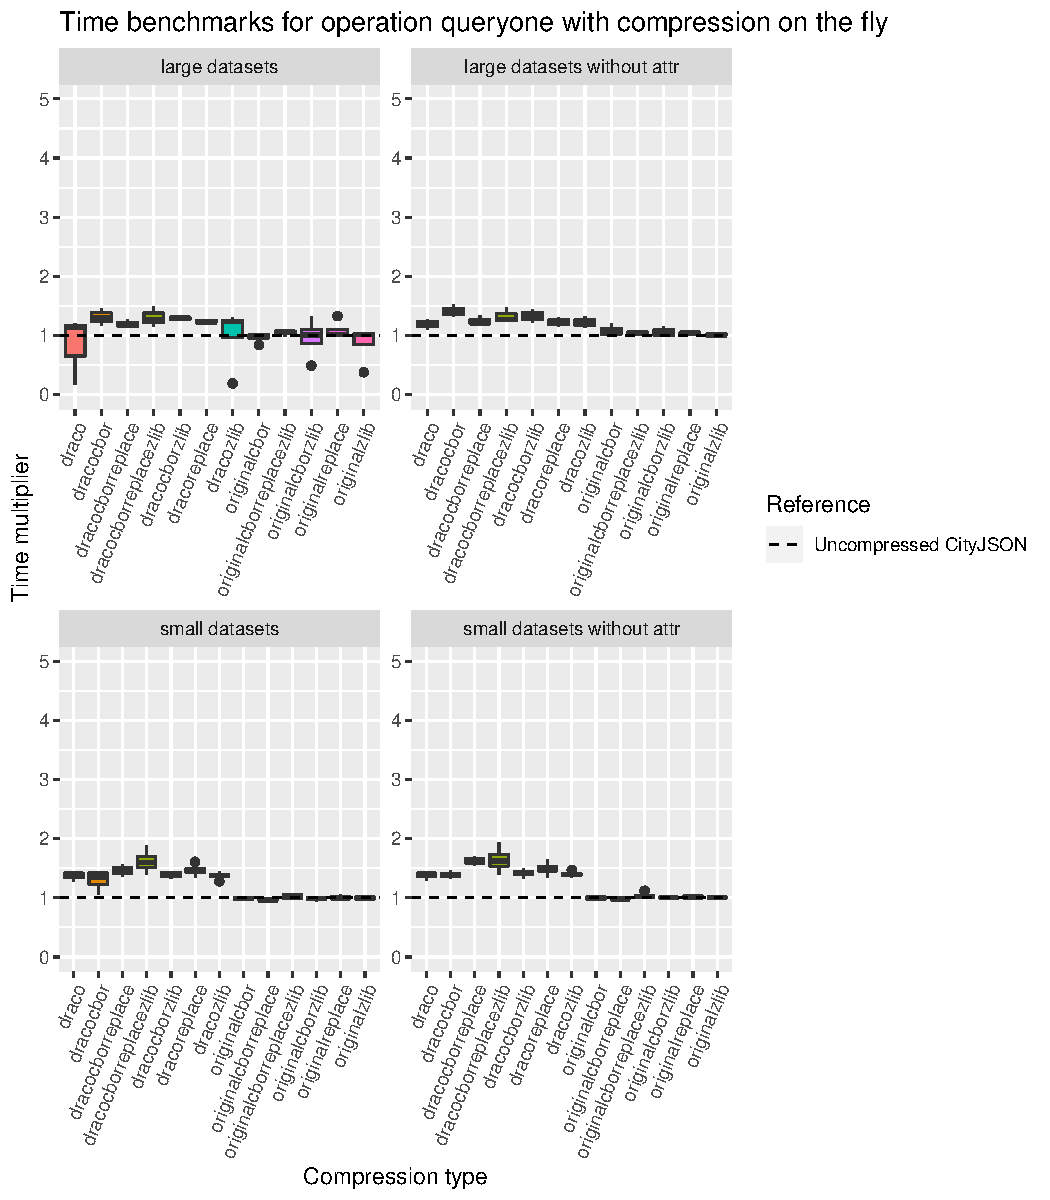
\includegraphics[scale=0.92]{figs/benchmark/individualotf/queryone.pdf}
    \caption{Boxplots of time performance of (on the fly) compressed datasets on querying one feature compared to uncompressed CityJSON.}
    \label{figotf:sdvis}
\end{figure}

For this use case, Draco compression is detrimental for performance.
Compression time is added into it and this is not worth it when compressing only one city object.
Other compression types are also often not worth it, especially on the large datasets, regardless of attributes.
With the small datasets, only original-cbor-replace works well with both dataset types.
One city object would not have much redundancy to compress and is already slim, so compression is not useful here and might even give slower performance.

On the fly compression can improve the querying time of CityJSON datasets on one city object to 100\%, 100\%, 96\%, or 98\% (when respectively using large datasets, large datasets without attributes, small datasets, and small datasets without attributes) of the time that it takes to perform the same operation with uncompressed CityJSON.


  \begin{table}[!h]
    \begin{minipage}{.5\linewidth}
      \caption{
Median performance with queryone on large datasets, compression on the fly}
\centering

\begin{tabular}{|l|r|}
\hline
Compression type & median\\
\hline
originalcbor & 1.005\\
\hline
originalcborzlib & 1.010\\
\hline
originalzlib & 1.015\\
\hline
originalreplace & 1.020\\
\hline
originalcborreplacezlib & 1.070\\
\hline
draco & 1.140\\
\hline
dracocborreplace & 1.180\\
\hline
dracoreplace & 1.230\\
\hline
dracozlib & 1.235\\
\hline
dracocborreplacezlib & 1.270\\
\hline
dracocborzlib & 1.300\\
\hline
dracocbor & 1.310\\
\hline
\end{tabular}
\end{minipage}%
    \begin{minipage}{.5\linewidth}
      \centering
        \caption{
Median performance with queryone on large datasets without attributes, compression on the fly}

\begin{tabular}{|l|r|}
\hline
Compression type & median\\
\hline
originalzlib & 1.010\\
\hline
originalcborzlib & 1.030\\
\hline
originalcborreplacezlib & 1.040\\
\hline
originalreplace & 1.040\\
\hline
originalcbor & 1.050\\
\hline
draco & 1.195\\
\hline
dracocborreplace & 1.210\\
\hline
dracoreplace & 1.220\\
\hline
dracozlib & 1.220\\
\hline
dracocborreplacezlib & 1.270\\
\hline
dracocborzlib & 1.330\\
\hline
dracocbor & 1.390\\
\hline
\end{tabular}
\end{minipage} 
\end{table}
\begin{table}[!h]
    \begin{minipage}{.5\linewidth}
      \caption{
Median performance with queryone on small datasets, compression on the fly}
\centering

\begin{tabular}{|l|r|}
\hline
Compression type & median\\
\hline
originalcborreplace & 0.960\\
\hline
originalcbor & 0.985\\
\hline
originalcborzlib & 0.990\\
\hline
originalzlib & 0.995\\
\hline
originalreplace & 1.000\\
\hline
originalcborreplacezlib & 1.020\\
\hline
dracocbor & 1.355\\
\hline
dracozlib & 1.380\\
\hline
draco & 1.400\\
\hline
dracocborzlib & 1.400\\
\hline
dracoreplace & 1.455\\
\hline
dracocborreplace & 1.460\\
\hline
dracocborreplacezlib & 1.595\\
\hline
\end{tabular}
\end{minipage}%
    \begin{minipage}{.5\linewidth}
      \centering
        \caption{
Median performance with queryone on small datasets without attributes, compression on the fly}

\begin{tabular}{|l|r|}
\hline
Compression type & median\\
\hline
originalcborreplace & 0.980\\
\hline
originalcbor & 1.000\\
\hline
originalcborzlib & 1.005\\
\hline
originalzlib & 1.005\\
\hline
originalreplace & 1.015\\
\hline
originalcborreplacezlib & 1.020\\
\hline
dracocbor & 1.390\\
\hline
dracozlib & 1.390\\
\hline
draco & 1.410\\
\hline
dracocborzlib & 1.425\\
\hline
dracoreplace & 1.495\\
\hline
dracocborreplace & 1.625\\
\hline
dracocborreplacezlib & 1.625\\
\hline
\end{tabular}
\end{minipage} 
\end{table}





\subsection{Querying all features}

\subsubsection{Compression in advance}

\begin{figure}[h!]
    %\hspace*{-2.3cm}  
    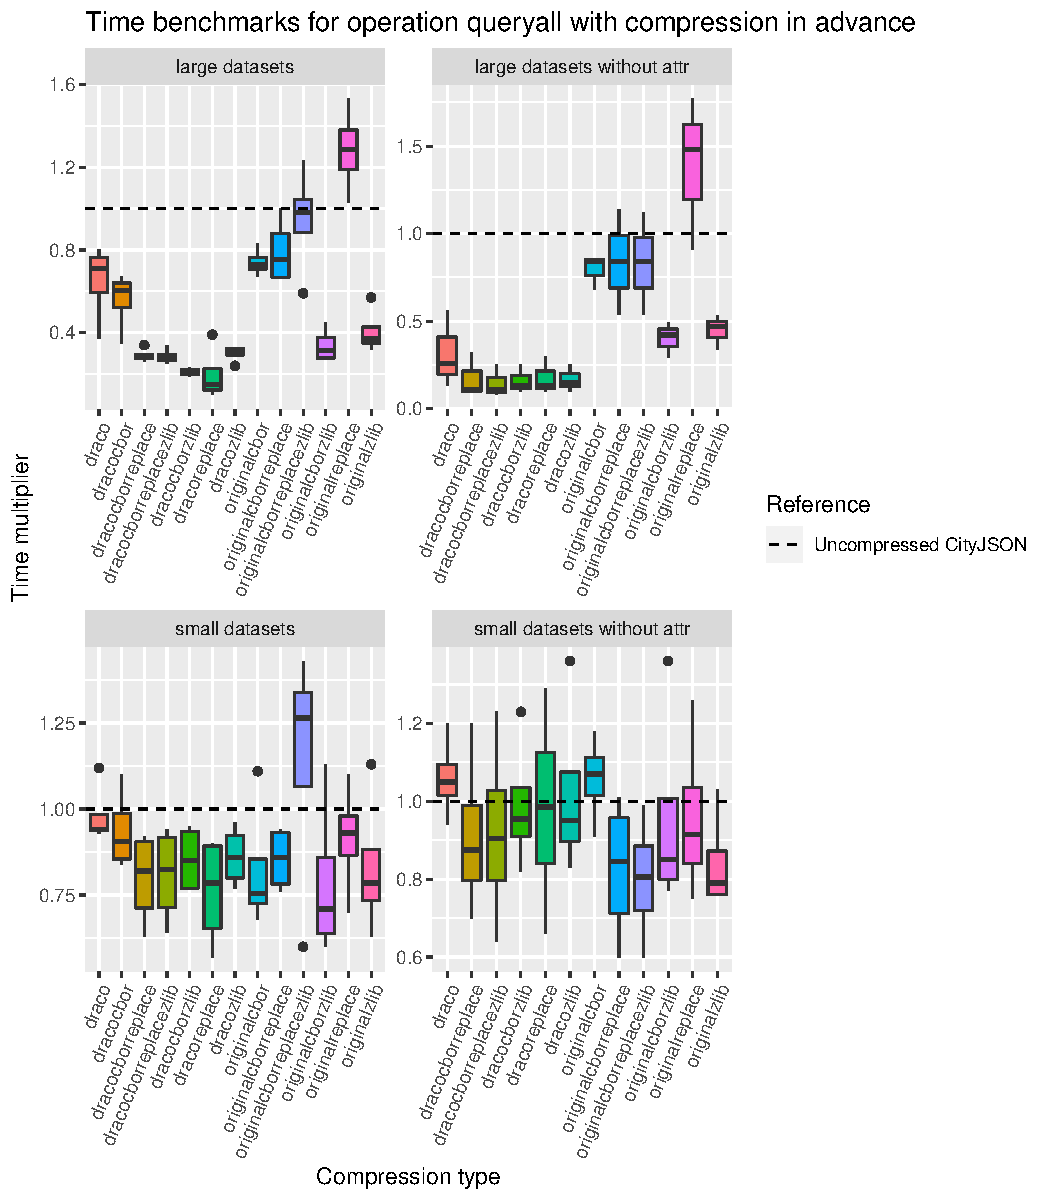
\includegraphics[scale=0.92]{figs/benchmark/individual/queryall.pdf}
    \caption{Boxplots of time performance of (in advance) compressed datasets on querying all features compared to uncompressed CityJSON.}
    \label{fig:sdvis}
\end{figure}

When querying all city objects, the whole dataset is traversed but the compression is performed on the complete file in the end.
With large datasets, using Draco is beneficial compared to compression types that do not use it.
This is likely due to Draco geometries being queried in a different way, as explained in Section~\ref{sec:queryone}.
However, original-cbor-zlib and original-zlib are also good, and are better than using draco alone or draco-cbor with datasets that have attributes.

As for the small datasets, Draco again provides less added benefits as is generally the case when datasets are compressed beforehand.
There is no clear pattern to be noted when comparing compression types to each other.
But as seen before as well, using cbor, zlib, or combinations of these prove to do well.

Compression in advance can improve the querying time of CityJSON datasets on all city objects to 15\%, 11\%, 71\%, or 79\% (when respectively using large datasets, large datasets without attributes, small datasets, and small datasets without attributes) of the time that it takes to perform the same operation with uncompressed CityJSON.



  \begin{table}[!h]
    \begin{minipage}{.5\linewidth}
      \caption{
Median performance with queryall on large datasets, compression in advance}
\centering

\begin{tabular}{|l|r|}
\hline
Compression type & median\\
\hline
dracoreplace & 0.150\\
\hline
dracocborzlib & 0.210\\
\hline
dracocborreplacezlib & 0.275\\
\hline
dracocborreplace & 0.280\\
\hline
dracozlib & 0.315\\
\hline
originalcborzlib & 0.315\\
\hline
originalzlib & 0.370\\
\hline
dracocbor & 0.605\\
\hline
draco & 0.710\\
\hline
originalcbor & 0.730\\
\hline
originalcborreplace & 0.755\\
\hline
originalcborreplacezlib & 0.980\\
\hline
originalreplace & 1.285\\
\hline
\end{tabular}
\end{minipage}%
    \begin{minipage}{.5\linewidth}
      \centering
        \caption{
Median performance with queryall on large datasets without attributes, compression in advance}

\begin{tabular}{|l|r|}
\hline
Compression type & median\\
\hline
dracocborreplace & 0.11\\
\hline
dracocborreplacezlib & 0.11\\
\hline
dracocborzlib & 0.13\\
\hline
dracoreplace & 0.13\\
\hline
dracozlib & 0.15\\
\hline
draco & 0.26\\
\hline
originalcborzlib & 0.42\\
\hline
originalzlib & 0.47\\
\hline
originalcbor & 0.84\\
\hline
originalcborreplace & 0.84\\
\hline
originalcborreplacezlib & 0.84\\
\hline
originalreplace & 1.48\\
\hline
\end{tabular}
\end{minipage} 
\end{table}
\begin{table}[!h]
    \begin{minipage}{.5\linewidth}
      \caption{
Median performance with queryall on small datasets, compression in advance}
\centering

\begin{tabular}{|l|r|}
\hline
Compression type & median\\
\hline
originalcborzlib & 0.710\\
\hline
originalcbor & 0.755\\
\hline
dracoreplace & 0.785\\
\hline
originalzlib & 0.785\\
\hline
dracocborreplace & 0.820\\
\hline
dracocborreplacezlib & 0.825\\
\hline
dracocborzlib & 0.850\\
\hline
dracozlib & 0.860\\
\hline
originalcborreplace & 0.860\\
\hline
dracocbor & 0.905\\
\hline
originalreplace & 0.930\\
\hline
draco & 0.940\\
\hline
originalcborreplacezlib & 1.265\\
\hline
\end{tabular}
\end{minipage}%
    \begin{minipage}{.5\linewidth}
      \centering
        \caption{
Median performance with queryall on small datasets without attributes, compression in advance}

\begin{tabular}{|l|r|}
\hline
Compression type & median\\
\hline
originalzlib & 0.790\\
\hline
originalcborreplacezlib & 0.805\\
\hline
originalcborreplace & 0.845\\
\hline
originalcborzlib & 0.850\\
\hline
dracocborreplace & 0.875\\
\hline
dracocborreplacezlib & 0.905\\
\hline
originalreplace & 0.915\\
\hline
dracozlib & 0.950\\
\hline
dracocborzlib & 0.955\\
\hline
dracoreplace & 0.985\\
\hline
draco & 1.050\\
\hline
originalcbor & 1.070\\
\hline
\end{tabular}
\end{minipage} 
\end{table}

\clearpage

\subsubsection{Compression on the fly}

\begin{figure}[h!]
    %\hspace*{-2.3cm}  
    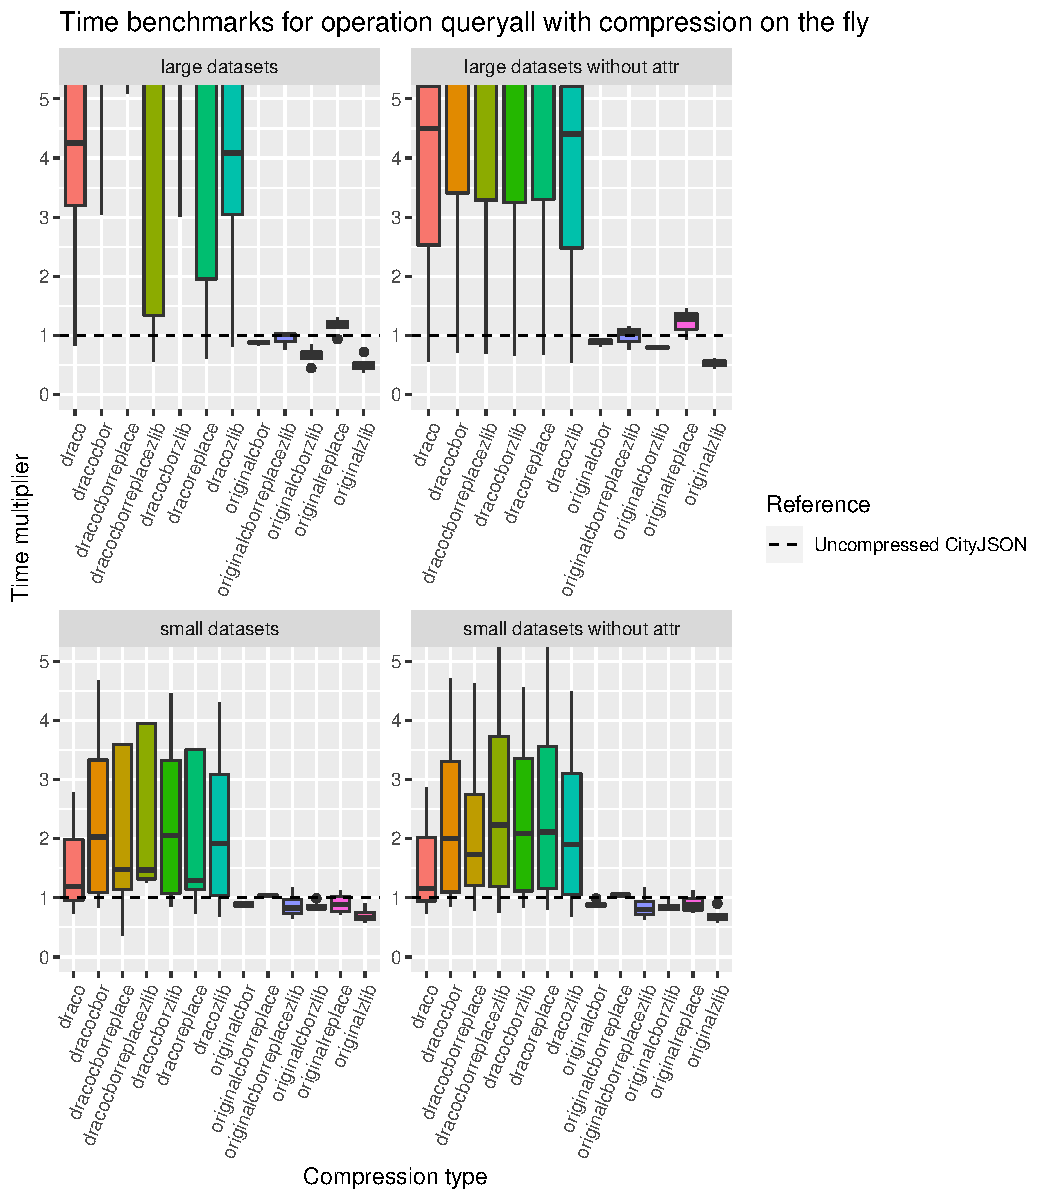
\includegraphics[scale=0.92]{figs/benchmark/individualotf/queryall.pdf}
    \caption{Boxplots of time performance of (on the fly) compressed datasets on querying all features compared to uncompressed CityJSON.}
    \label{figotf:sdvis}
\end{figure}

The graphs are limited by a time multiplier of 5.
Again, using Draco is not a good idea when compressing datasets on the fly because of the relatively high compression time.
Original-replace is unsuitable with large datasets, and original-cbor-replace-zlib also does not do very well.
Original-zlib and original-cbor-zlib are the best ones, both with and without attributes.
As for the small datasets these two are also good, but using the replace method is now not noticeably worse.

On the fly compression can improve the querying time of CityJSON datasets on all city objects to 47\%, 53\%, 67\%, or 65\% (when respectively using large datasets, large datasets without attributes, small datasets, and small datasets without attributes) of the time that it takes to perform the same operation with uncompressed CityJSON.


\begin{table}[!h]
    \begin{minipage}{.5\linewidth}
      \caption{
Median performance with queryall on large datasets, compression on the fly}
\centering

\begin{tabular}{|l|r|}
\hline
Compression type & median\\
\hline
originalzlib & 0.470\\
\hline
originalcborzlib & 0.675\\
\hline
originalcbor & 0.885\\
\hline
originalcborreplacezlib & 1.020\\
\hline
originalreplace & 1.205\\
\hline
dracozlib & 4.085\\
\hline
draco & 4.255\\
\hline
dracoreplace & 6.125\\
\hline
dracocborreplacezlib & 6.340\\
\hline
dracocborzlib & 7.465\\
\hline
dracocbor & 9.835\\
\hline
dracocborreplace & 13.260\\
\hline
\end{tabular}
\end{minipage}%
    \begin{minipage}{.5\linewidth}
      \centering
        \caption{
Median performance with queryall on large datasets without attributes, compression on the fly}

\begin{tabular}{|l|r|}
\hline
Compression type & median\\
\hline
originalzlib & 0.53\\
\hline
originalcborzlib & 0.80\\
\hline
originalcbor & 0.91\\
\hline
originalcborreplacezlib & 1.04\\
\hline
originalreplace & 1.28\\
\hline
dracozlib & 4.41\\
\hline
draco & 4.50\\
\hline
dracocborzlib & 5.82\\
\hline
dracocborreplacezlib & 5.88\\
\hline
dracoreplace & 5.93\\
\hline
dracocbor & 6.11\\
\hline
\end{tabular}
\end{minipage} 
\end{table}
\begin{table}[!h]
    \begin{minipage}{.5\linewidth}
      \caption{
Median performance with queryall on small datasets, compression on the fly}
\centering

\begin{tabular}{|l|r|}
\hline
Compression type & median\\
\hline
originalzlib & 0.670\\
\hline
originalcborzlib & 0.820\\
\hline
originalcborreplacezlib & 0.830\\
\hline
originalcbor & 0.890\\
\hline
originalreplace & 0.890\\
\hline
originalcborreplace & 1.040\\
\hline
draco & 1.190\\
\hline
dracoreplace & 1.290\\
\hline
dracocborreplacezlib & 1.470\\
\hline
dracocborreplace & 1.475\\
\hline
dracozlib & 1.920\\
\hline
dracocbor & 2.030\\
\hline
dracocborzlib & 2.050\\
\hline
\end{tabular}
\end{minipage}%     
    \begin{minipage}{.5\linewidth}
      \centering
        \caption{
Median performance with queryall on small datasets without attributes, compression on the fly}

\begin{tabular}{|l|r|}
\hline
Compression type & median\\
\hline
originalzlib & 0.650\\
\hline
originalcborreplacezlib & 0.805\\
\hline
originalcborzlib & 0.820\\
\hline
originalcbor & 0.870\\
\hline
originalreplace & 0.880\\
\hline
originalcborreplace & 1.050\\
\hline
draco & 1.160\\
\hline
dracocborreplace & 1.735\\
\hline
dracozlib & 1.905\\
\hline
dracocbor & 2.005\\
\hline
dracocborzlib & 2.085\\
\hline
dracoreplace & 2.115\\
\hline
dracocborreplacezlib & 2.230\\
\hline
\end{tabular}
\end{minipage} 
\end{table}

\newpage

\section{Spatial analysis}
\label{bmbuffering}

\subsection{Buffering one feature}


\subsubsection{Compression in advance}

\begin{figure}[h!]
    %\hspace*{-2.3cm}  
    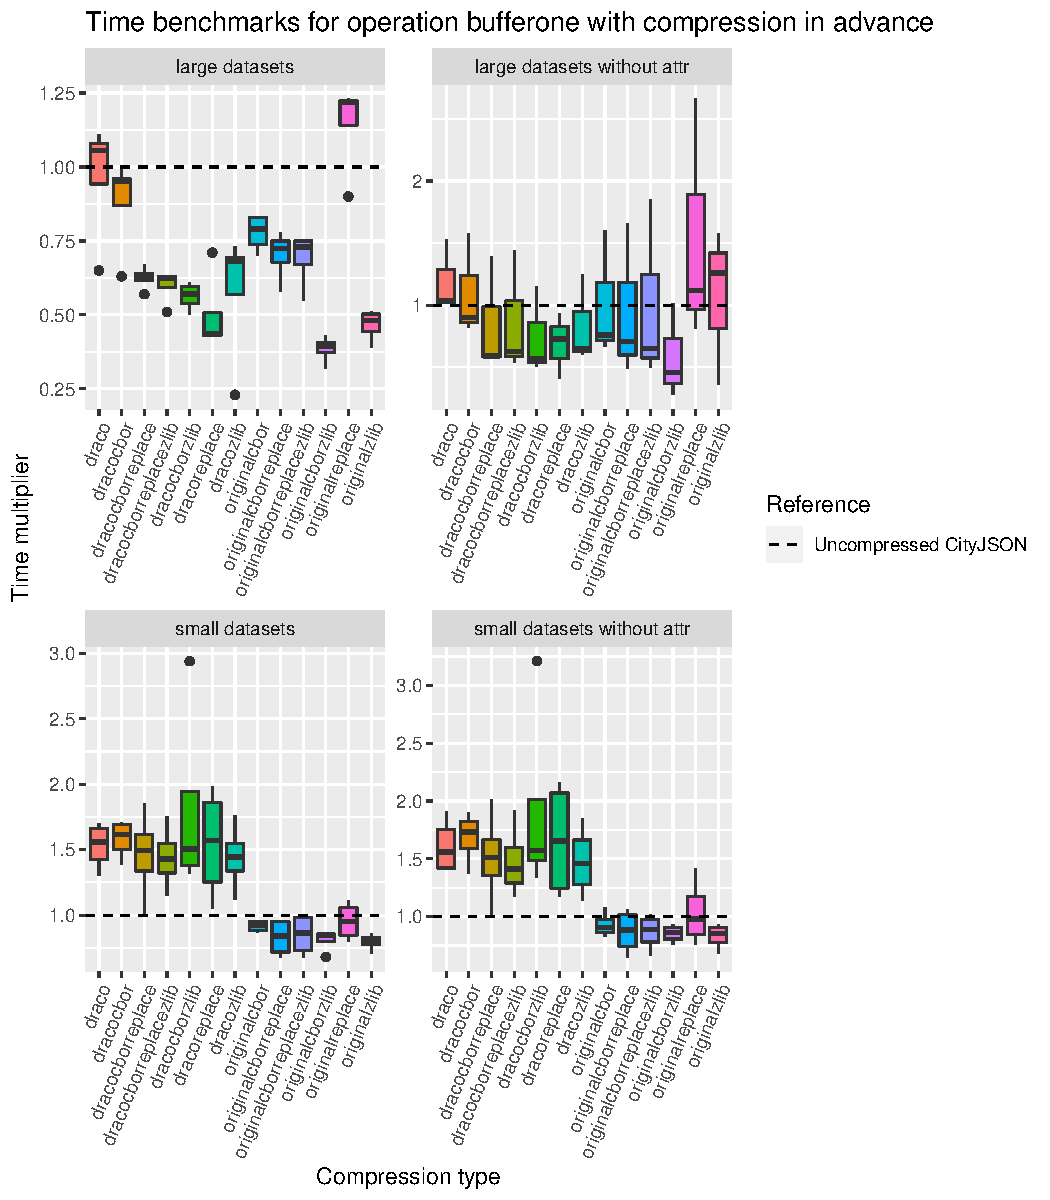
\includegraphics[scale=0.92]{figs/benchmark/individual/bufferone.pdf}
    \caption{Boxplots of time performance of (in advance) compressed datasets on buffering one feature compared to uncompressed CityJSON.}
    \label{fig:sdvis}
\end{figure}

Draco geometries are handled in a different way than original geometries as explained in Section~\ref{sec:implbufferone}.
Despite that, for the large datasets it is not easy to see whether it is better to use it or not.
There are also no clear rends to be seen, except for that original-replace is bad both with and without attributes, and original-cbor-zlib is the best option for both of these dataset types.
In general, most compression types work well with large datasets with attributes but not as good when attributes are not included.
In the latter case both attribute and JSON compression techniques have less data to compress, which might make them less effective.
Regarding the small datasets, the use of Draco gives worse results than not using it due to overhead.
The other compression types general do well as compared to the baseline, except for original-replace.

Compression in advance can improve the buffering time of CityJSON datasets on one city object to 39\%, 46\%, 81\%, or 85\% (when respectively using large datasets, large datasets without attributes, small datasets, and small datasets without attributes) of the time that it takes to perform the same operation with uncompressed CityJSON.



  \begin{table}[!h]
    \begin{minipage}{.5\linewidth}
      \caption{
Median performance with bufferone on large datasets, compression in advance}
\centering

\begin{tabular}{|l|r|}
\hline
Compression type & median\\
\hline
originalcborzlib & 0.395\\
\hline
dracoreplace & 0.435\\
\hline
originalzlib & 0.480\\
\hline
dracocborzlib & 0.570\\
\hline
dracocborreplacezlib & 0.625\\
\hline
dracocborreplace & 0.630\\
\hline
dracozlib & 0.680\\
\hline
originalcborreplace & 0.725\\
\hline
originalcborreplacezlib & 0.730\\
\hline
originalcbor & 0.790\\
\hline
dracocbor & 0.950\\
\hline
draco & 1.055\\
\hline
originalreplace & 1.220\\
\hline
\end{tabular}
\end{minipage}%
    \begin{minipage}{.5\linewidth}
      \centering
        \caption{
Median performance with bufferone on large datasets without attributes, compression in advance}

\begin{tabular}{|l|r|}
\hline
Compression type & median\\
\hline
originalcborzlib & 0.46\\
\hline
dracocborzlib & 0.57\\
\hline
dracocborreplace & 0.59\\
\hline
dracocborreplacezlib & 0.63\\
\hline
dracozlib & 0.65\\
\hline
originalcborreplacezlib & 0.65\\
\hline
originalcborreplace & 0.71\\
\hline
dracoreplace & 0.73\\
\hline
originalcbor & 0.76\\
\hline
dracocbor & 0.90\\
\hline
draco & 1.04\\
\hline
originalreplace & 1.12\\
\hline
originalzlib & 1.26\\
\hline
\end{tabular}
\end{minipage} 
\end{table}
\begin{table}[!h]
    \begin{minipage}{.5\linewidth}
      \caption{
Median performance with bufferone on small datasets, compression in advance}
\centering

\begin{tabular}{|l|r|}
\hline
Compression type & median\\
\hline
originalzlib & 0.810\\
\hline
originalcborreplace & 0.840\\
\hline
originalcborzlib & 0.845\\
\hline
originalcborreplacezlib & 0.865\\
\hline
originalcbor & 0.920\\
\hline
originalreplace & 0.950\\
\hline
dracocborreplacezlib & 1.430\\
\hline
dracozlib & 1.445\\
\hline
dracocborreplace & 1.495\\
\hline
dracocborzlib & 1.505\\
\hline
draco & 1.560\\
\hline
dracoreplace & 1.570\\
\hline
dracocbor & 1.615\\
\hline
\end{tabular}
\end{minipage}%
    \begin{minipage}{.5\linewidth}
      \centering
        \caption{
Median performance with bufferone on small datasets without attributes, compression in advance}

\begin{tabular}{|l|r|}
\hline
Compression type & median\\
\hline
originalzlib & 0.855\\
\hline
originalcborzlib & 0.860\\
\hline
originalcborreplace & 0.885\\
\hline
originalcborreplacezlib & 0.890\\
\hline
originalcbor & 0.905\\
\hline
originalreplace & 0.980\\
\hline
dracocborreplacezlib & 1.410\\
\hline
dracozlib & 1.460\\
\hline
dracocborreplace & 1.510\\
\hline
draco & 1.560\\
\hline
dracocborzlib & 1.570\\
\hline
dracoreplace & 1.655\\
\hline
dracocbor & 1.730\\
\hline
\end{tabular}
\end{minipage} 
\end{table}



\subsubsection{Compression on the fly}

\begin{figure}[h!]
    %\hspace*{-2.3cm}  
    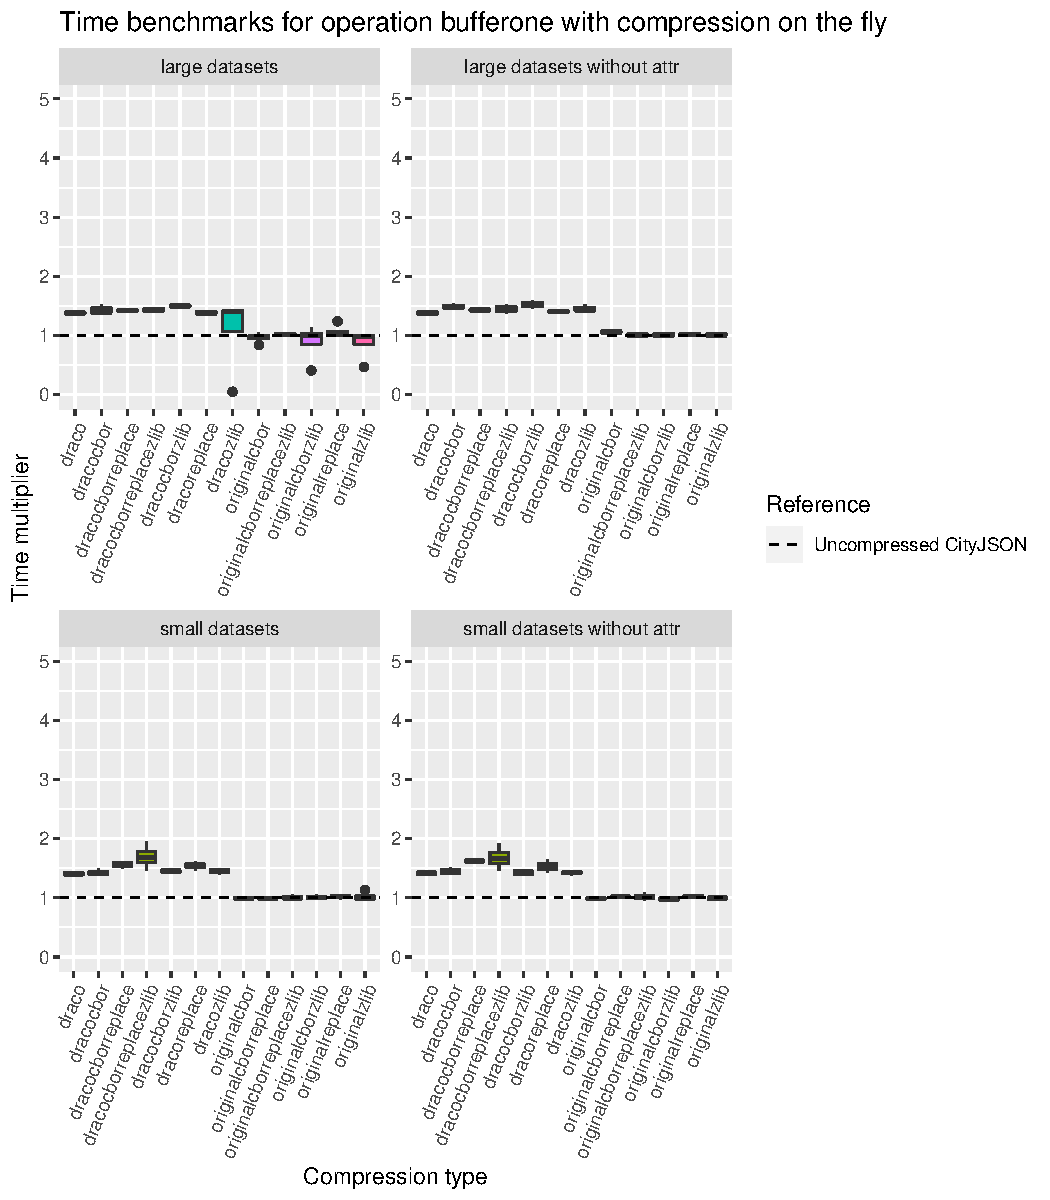
\includegraphics[scale=0.92]{figs/benchmark/individualotf/bufferone.pdf}
    \caption{Boxplots of time performance of (on the fly) compressed datasets on buffering one feature compared to uncompressed CityJSON.}
    \label{figotf:sdvis}
\end{figure}

As opposed to compressing in advance, it is almost never worth it to compress buffer data on the fly since the medians of the boxplots are above the baseline or very slightly underneath it.
This means that the added compression time is not outweighed by the faster transmission of the data.
Especially when using Draco this is true.
When using a compression type that retains original geometries, the results can be neutral so it is at least still fine to implement such kind of compression.

On the fly compression can improve the buffering time of CityJSON datasets on one city object to 98\%, 100\%, 99\%, or 98\% (when respectively using large datasets, large datasets without attributes, small datasets, and small datasets without attributes) of the time that it takes to perform the same operation with uncompressed CityJSON.


  \begin{table}[!h]
    \begin{minipage}{.5\linewidth}
      \caption{
Median performance with bufferone on large datasets, compression on the fly}
\centering

\begin{tabular}{|l|r|}
\hline
Compression type & median\\
\hline
originalcbor & 0.980\\
\hline
originalzlib & 0.985\\
\hline
originalcborzlib & 1.000\\
\hline
originalreplace & 1.015\\
\hline
originalcborreplacezlib & 1.020\\
\hline
draco & 1.380\\
\hline
dracoreplace & 1.380\\
\hline
dracocbor & 1.400\\
\hline
dracozlib & 1.410\\
\hline
dracocborreplace & 1.420\\
\hline
dracocborreplacezlib & 1.430\\
\hline
dracocborzlib & 1.500\\
\hline
\end{tabular}
\end{minipage}%
    \begin{minipage}{.5\linewidth}
      \centering
        \caption{
Median performance with bufferone on large datasets without attributes, compression on the fly}

\begin{tabular}{|l|r|}
\hline
Compression type & median\\
\hline
originalcborzlib & 1.000\\
\hline
originalcborreplacezlib & 1.010\\
\hline
originalzlib & 1.010\\
\hline
originalreplace & 1.020\\
\hline
originalcbor & 1.060\\
\hline
draco & 1.385\\
\hline
dracoreplace & 1.410\\
\hline
dracocborreplace & 1.430\\
\hline
dracozlib & 1.430\\
\hline
dracocborreplacezlib & 1.440\\
\hline
dracocbor & 1.480\\
\hline
dracocborzlib & 1.520\\
\hline
\end{tabular}
\end{minipage} 
\end{table}
\begin{table}[!h]
    \begin{minipage}{.5\linewidth}
      \caption{
Median performance with bufferone on small datasets, compression on the fly}
\centering

\begin{tabular}{|l|r|}
\hline
Compression type & median\\
\hline
originalcbor & 0.990\\
\hline
originalcborreplace & 0.990\\
\hline
originalzlib & 0.995\\
\hline
originalcborreplacezlib & 1.000\\
\hline
originalcborzlib & 1.005\\
\hline
originalreplace & 1.025\\
\hline
draco & 1.400\\
\hline
dracocbor & 1.415\\
\hline
dracocborzlib & 1.450\\
\hline
dracozlib & 1.455\\
\hline
dracoreplace & 1.545\\
\hline
dracocborreplace & 1.560\\
\hline
dracocborreplacezlib & 1.680\\
\hline
\end{tabular}
\end{minipage}%       
    \begin{minipage}{.5\linewidth}
      \centering
        \caption{
Median performance with bufferone on small datasets without attributes, compression on the fly}

\begin{tabular}{|l|r|}
\hline
Compression type & median\\
\hline
originalcborzlib & 0.980\\
\hline
originalcbor & 0.985\\
\hline
originalzlib & 0.995\\
\hline
originalcborreplacezlib & 1.005\\
\hline
originalcborreplace & 1.020\\
\hline
originalreplace & 1.020\\
\hline
draco & 1.420\\
\hline
dracocborzlib & 1.425\\
\hline
dracozlib & 1.425\\
\hline
dracocbor & 1.440\\
\hline
dracoreplace & 1.525\\
\hline
dracocborreplace & 1.625\\
\hline
dracocborreplacezlib & 1.665\\
\hline
\end{tabular}
\end{minipage} 
\end{table}

\newpage

\subsection{Buffering all features}
\label{resultsbufferall}

\subsubsection{Compression in advance}

\begin{figure}[h!]
    %\hspace*{-2.3cm}  
    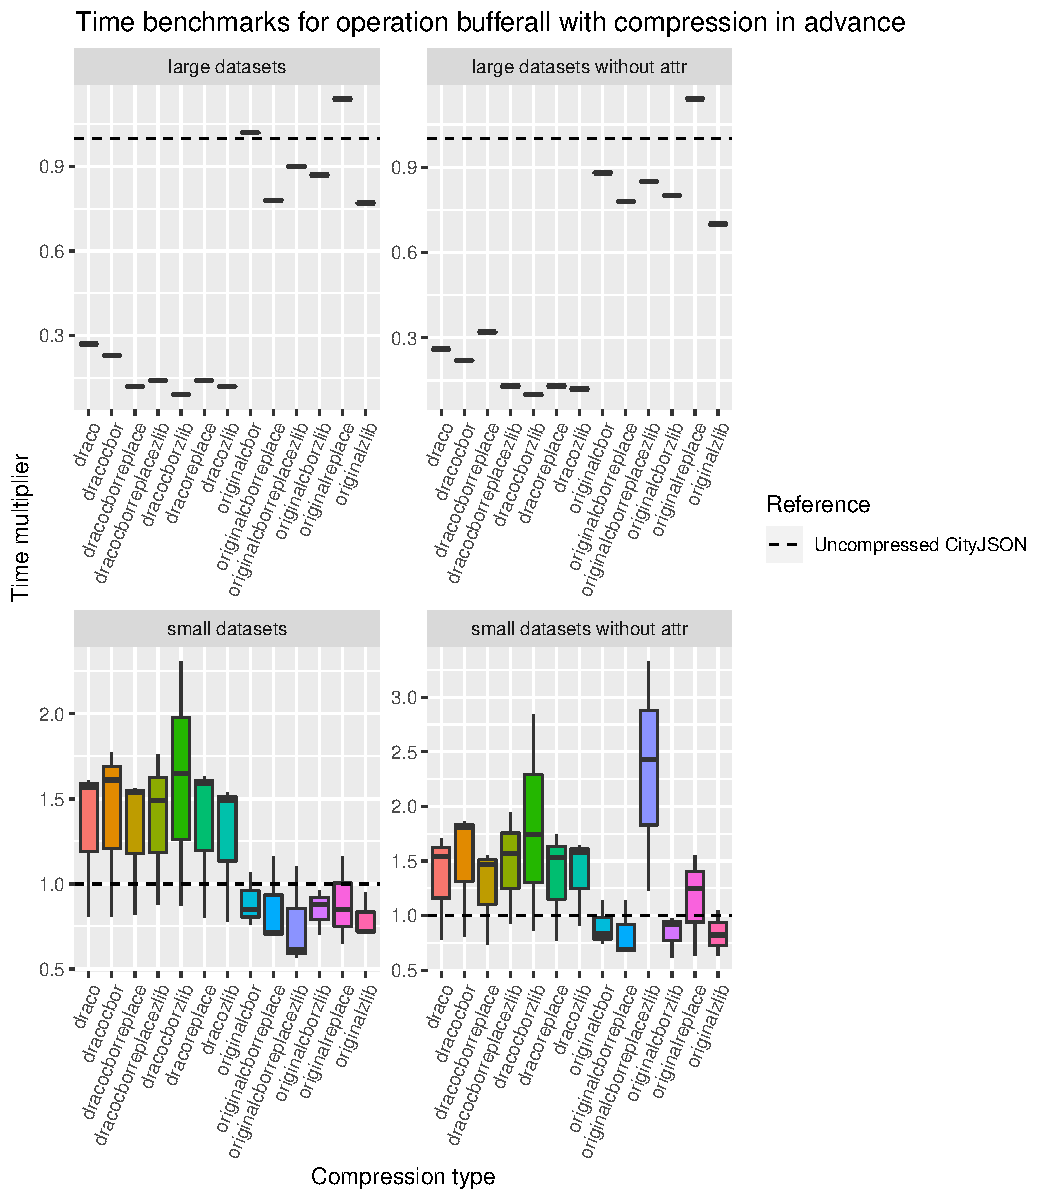
\includegraphics[scale=0.92]{figs/benchmark/individual/bufferall.pdf}
    \caption{Boxplots of time performance of (in advance) compressed datasets on buffering all features compared to uncompressed CityJSON.}
    \label{fig:sdvis}
\end{figure}

When buffering all features in the client, using Draco is clearly a good idea for the large datasets.
Draco geometries are buffered in a different way (see Section~\ref{sec:implbufferone}), and this shows a more apparent advantage when all geometries are buffered instead of one.
Compression types without it generally still improve the performance in comparison to the baseline, but not as much.
For small datasets these perform better however, which is also seen with the other use cases with small datasets.
Draco is again unsuitable to use with those.
But ultimately, it is questionable whether or not it is wise to use compression at all for this use case, since the boxplots show that most compression types that have a median below the baseline still have their boxplots touching or above the baseline.

Compression in advance can improve the buffering time of CityJSON datasets on all city objects to 9\%, 10\%, 61\%, or 69\% (when respectively using large datasets, large datasets without attributes, small datasets, and small datasets without attributes) of the time that it takes to perform the same operation with uncompressed CityJSON.



  \begin{table}[!h]
    \begin{minipage}{.5\linewidth}
      \caption{
Median performance with bufferall on large datasets, compression in advance}
\centering

\begin{tabular}{|l|r|}
\hline
Compression type & median\\
\hline
dracocborzlib & 0.09\\
\hline
dracocborreplace & 0.12\\
\hline
dracozlib & 0.12\\
\hline
dracocborreplacezlib & 0.14\\
\hline
dracoreplace & 0.14\\
\hline
dracocbor & 0.23\\
\hline
draco & 0.27\\
\hline
originalzlib & 0.77\\
\hline
originalcborreplace & 0.78\\
\hline
originalcborzlib & 0.87\\
\hline
originalcborreplacezlib & 0.90\\
\hline
originalcbor & 1.02\\
\hline
originalreplace & 1.14\\
\hline
\end{tabular}
\end{minipage}%
    \begin{minipage}{.5\linewidth}
      \centering
        \caption{
Median performance with bufferall on large datasets without attributes, compression in advance}

\begin{tabular}{|l|r|}
\hline
Compression type & median\\
\hline
dracocborzlib & 0.10\\
\hline
dracozlib & 0.12\\
\hline
dracocborreplacezlib & 0.13\\
\hline
dracoreplace & 0.13\\
\hline
dracocbor & 0.22\\
\hline
draco & 0.26\\
\hline
dracocborreplace & 0.32\\
\hline
originalzlib & 0.70\\
\hline
originalcborreplace & 0.78\\
\hline
originalcborzlib & 0.80\\
\hline
originalcborreplacezlib & 0.85\\
\hline
originalcbor & 0.88\\
\hline
originalreplace & 1.14\\
\hline
\end{tabular}
\end{minipage} 
\end{table}
\begin{table}[!h]
    \begin{minipage}{.5\linewidth}
      \caption{
Median performance with bufferall on small datasets, compression in advance}
\centering

\begin{tabular}{|l|r|}
\hline
Compression type & median\\
\hline
originalcborreplacezlib & 0.61\\
\hline
originalcborreplace & 0.71\\
\hline
originalzlib & 0.72\\
\hline
originalcbor & 0.85\\
\hline
originalreplace & 0.85\\
\hline
originalcborzlib & 0.88\\
\hline
dracocborreplacezlib & 1.49\\
\hline
dracozlib & 1.49\\
\hline
dracocborreplace & 1.54\\
\hline
draco & 1.57\\
\hline
dracoreplace & 1.59\\
\hline
dracocbor & 1.61\\
\hline
dracocborzlib & 1.65\\
\hline
\end{tabular}
\end{minipage}%
    \begin{minipage}{.5\linewidth}
      \centering
        \caption{
Median performance with bufferall on small datasets without attributes, compression in advance}

\begin{tabular}{|l|r|}
\hline
Compression type & median\\
\hline
originalcborreplace & 0.69\\
\hline
originalzlib & 0.82\\
\hline
originalcbor & 0.83\\
\hline
originalcborzlib & 0.92\\
\hline
originalreplace & 1.25\\
\hline
dracocborreplace & 1.47\\
\hline
dracoreplace & 1.53\\
\hline
draco & 1.54\\
\hline
dracocborreplacezlib & 1.57\\
\hline
dracozlib & 1.58\\
\hline
dracocborzlib & 1.74\\
\hline
dracocbor & 1.81\\
\hline
originalcborreplacezlib & 2.43\\
\hline
\end{tabular}
\end{minipage} 
\end{table}

\clearpage

\subsubsection{Compression on the fly}

\begin{figure}[h!]
    %\hspace*{-2.3cm}  
    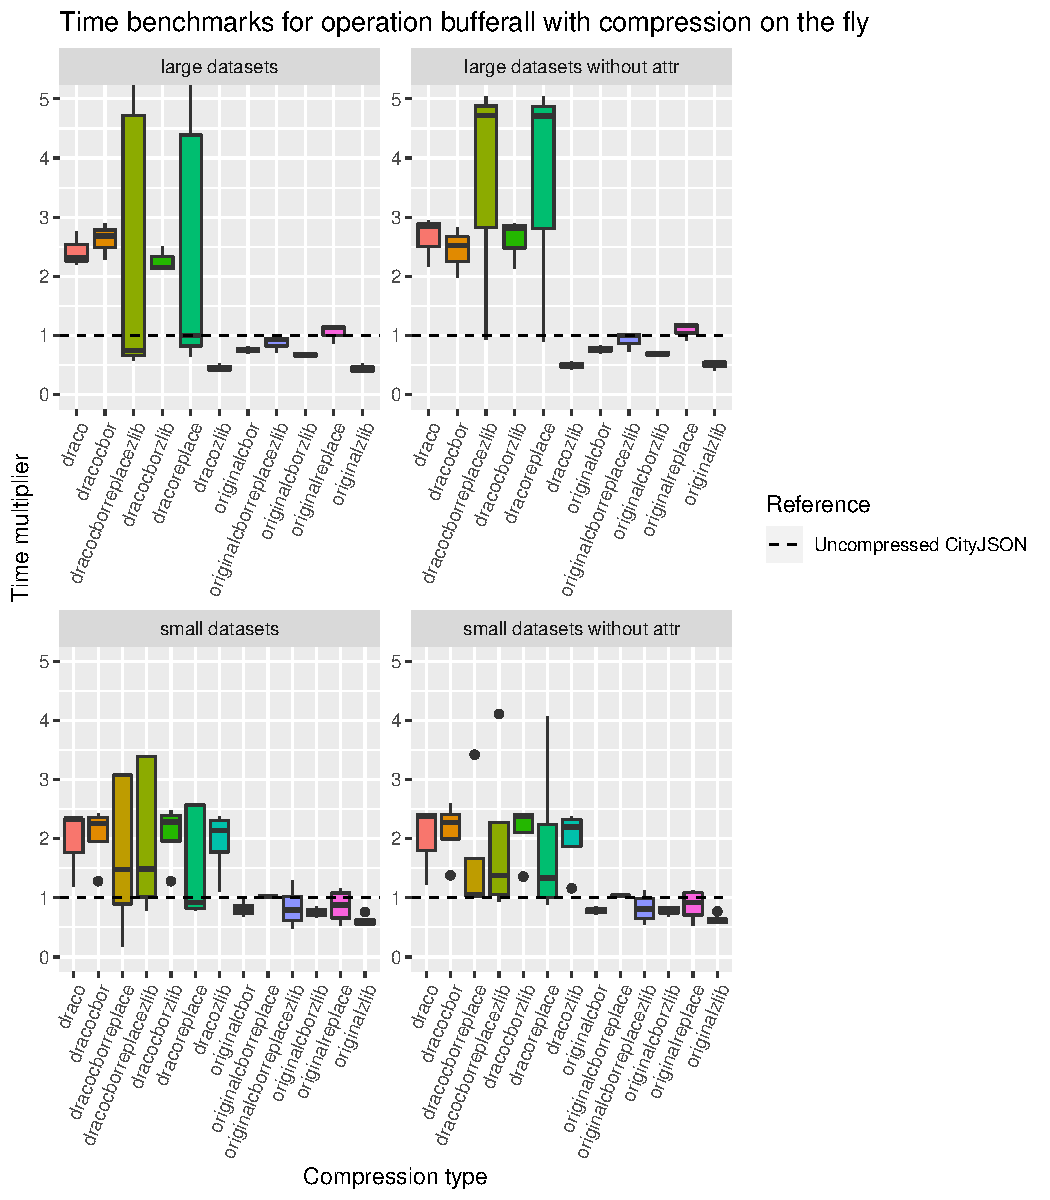
\includegraphics[scale=0.92]{figs/benchmark/individualotf/bufferall.pdf}
    \caption{Boxplots of time performance of (on the fly) compressed datasets on buffering all features compared to uncompressed CityJSON.}
    \label{figotf:sdvis}
\end{figure}

Using Draco compression on the fly is not useful.
Other compression types on the other hand do provide benefits, except when the replace method is used.
This is true for all dataset types, and there are no other interesting patterns to see in the graphs.


On the fly compression can improve the buffering time of CityJSON datasets on all city objects to 41\%, 50\%, 57\%, or 60\% (when respectively using large datasets, large datasets without attributes, small datasets, and small datasets without attributes) of the time that it takes to perform the same operation with uncompressed CityJSON.


\begin{table}[!h]
    \begin{minipage}{.5\linewidth}
      \caption{
Median performance with bufferall on large datasets, compression on the fly}
\centering

\begin{tabular}{|l|r|}
\hline
Compression type & median\\
\hline
originalzlib & 0.41\\
\hline
dracozlib & 0.43\\
\hline
originalcborzlib & 0.68\\
\hline
dracocborreplacezlib & 0.75\\
\hline
originalcbor & 0.76\\
\hline
originalcborreplacezlib & 0.93\\
\hline
dracoreplace & 1.00\\
\hline
originalreplace & 1.14\\
\hline
dracocborzlib & 2.15\\
\hline
draco & 2.32\\
\hline
dracocbor & 2.68\\
\hline
\end{tabular}
\end{minipage}%
    \begin{minipage}{.5\linewidth}
      \centering
        \caption{
Median performance with bufferall on large datasets without attributes, compression on the fly}

\begin{tabular}{|l|r|}
\hline
Compression type & median\\
\hline
dracozlib & 0.50\\
\hline
originalzlib & 0.54\\
\hline
originalcborzlib & 0.70\\
\hline
originalcbor & 0.77\\
\hline
originalcborreplacezlib & 1.00\\
\hline
originalreplace & 1.17\\
\hline
dracocbor & 2.52\\
\hline
dracocborzlib & 2.82\\
\hline
draco & 2.84\\
\hline
dracoreplace & 4.71\\
\hline
dracocborreplacezlib & 4.72\\
\hline
\end{tabular}
\end{minipage} 
\end{table}
\begin{table}[!h]
    \begin{minipage}{.5\linewidth}
      \caption{
Median performance with bufferall on small datasets, compression on the fly}
\centering

\begin{tabular}{|l|r|}
\hline
Compression type & median\\
\hline
originalzlib & 0.575\\
\hline
originalcborzlib & 0.750\\
\hline
originalcborreplacezlib & 0.795\\
\hline
originalcbor & 0.800\\
\hline
originalreplace & 0.880\\
\hline
dracoreplace & 0.925\\
\hline
originalcborreplace & 1.020\\
\hline
dracocborreplace & 1.475\\
\hline
dracocborreplacezlib & 1.485\\
\hline
dracozlib & 2.140\\
\hline
dracocbor & 2.260\\
\hline
dracocborzlib & 2.280\\
\hline
draco & 2.330\\
\hline
\end{tabular}
\end{minipage}%
    \begin{minipage}{.5\linewidth}
      \centering
        \caption{
Median performance with bufferall on small datasets without attributes, compression on the fly}

\begin{tabular}{|l|r|}
\hline
Compression type & median\\
\hline
originalzlib & 0.600\\
\hline
originalcbor & 0.785\\
\hline
originalcborzlib & 0.800\\
\hline
originalcborreplacezlib & 0.815\\
\hline
originalreplace & 0.920\\
\hline
originalcborreplace & 1.040\\
\hline
dracocborreplace & 1.060\\
\hline
dracoreplace & 1.335\\
\hline
dracocborreplacezlib & 1.375\\
\hline
dracozlib & 2.200\\
\hline
dracocbor & 2.270\\
\hline
dracocborzlib & 2.375\\
\hline
draco & 2.380\\
\hline
\end{tabular}
\end{minipage} 
\end{table}



\newpage

\section{Editing (attributes)}
\label{bmeditingattr}

\subsection{Editing attributes one feature}

\subsubsection{Compression in advance}

\begin{figure}[h!]
    %\hspace*{-2.3cm}  
    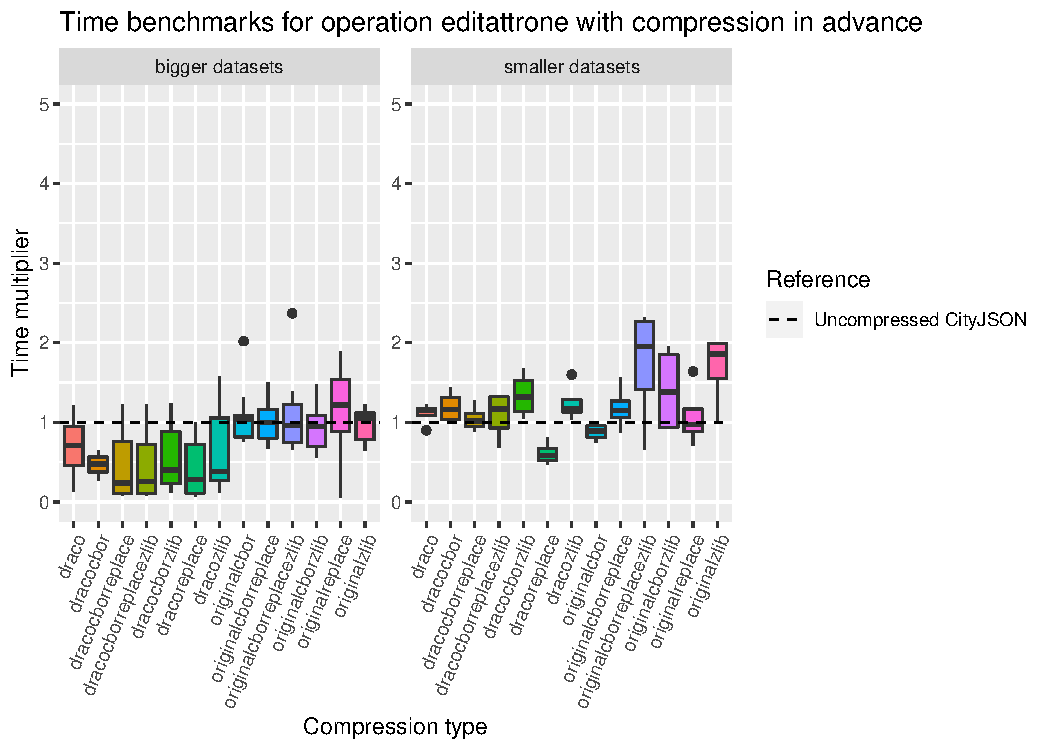
\includegraphics[scale=0.92]{figs/benchmark/individual/editattrone.pdf}
    \caption{Boxplots of time performance of (in advance) compressed datasets on editing attributes of one feature compared to uncompressed CityJSON.}
    \label{fig:sdvis}
\end{figure}

For this use case the compression time becomes relevant, as opposed to the other use cases with compression in advance.
Despite that, the results seem unexpectedly good.
When using Draco compression in combination with large datasets, the performance is rather well both compared to the baseline and to compression types without Draco.
That is because the Draco geometries are not touched as they are not edited, so they also do not need to be compressed again and they make for small file sizes, benefitting the transmission time.
The addition of other compression techniques is beneficial as well since using Draco only does not compare very well to the other Draco compression types.
When not using Draco original-cbor, original-cbor-zlib, and original-zlib do well.

With the small datasets most compression types are not suitable.
Draco-replace does work well which could be explained by the different way in which attributes can be edited with the replace method and the advantage of Draco as mentioned in the paragraph above, but other compression types using this method do not do particularly well. 
Original-cbor is also slightly better than the baseline.

Compression in advance can improve the attribute editing time of CityJSON datasets on one city object to 10\% or 58\% (when respectively using large datasets and small datasets) of the time that it takes to perform the same operation with uncompressed CityJSON.


  \begin{table}[!h]
    \begin{minipage}{.5\linewidth}
      \caption{
Median performance with editattrone on large datasets, compression in advance}
\centering

\begin{tabular}{|l|r|}
\hline
Compression type & median\\
\hline
dracoreplace & 0.100\\
\hline
dracocborreplace & 0.135\\
\hline
dracocborreplacezlib & 0.140\\
\hline
dracocborzlib & 0.335\\
\hline
dracozlib & 0.360\\
\hline
dracocbor & 0.475\\
\hline
originalcborzlib & 0.600\\
\hline
draco & 0.655\\
\hline
originalzlib & 0.730\\
\hline
originalcbor & 0.810\\
\hline
originalcborreplace & 1.015\\
\hline
originalcborreplacezlib & 1.135\\
\hline
originalreplace & 1.330\\
\hline
\end{tabular}
\end{minipage}%
    \begin{minipage}{.5\linewidth}
      \centering
        \caption{
Median performance with editattrone on small datasets, compression in advance}

\begin{tabular}{|l|r|}
\hline
Compression type & median\\
\hline
dracoreplace & 0.580\\
\hline
originalcbor & 0.890\\
\hline
originalreplace & 0.975\\
\hline
dracocborreplace & 1.015\\
\hline
originalcborreplace & 1.150\\
\hline
draco & 1.155\\
\hline
dracocbor & 1.160\\
\hline
dracocborreplacezlib & 1.165\\
\hline
dracozlib & 1.170\\
\hline
dracocborzlib & 1.320\\
\hline
originalcborzlib & 1.380\\
\hline
originalzlib & 1.860\\
\hline
originalcborreplacezlib & 1.955\\
\hline
\end{tabular}
\end{minipage} 
\end{table}



\subsubsection{Compression on the fly}

\begin{figure}[h!]
    %\hspace*{-2.3cm}  
    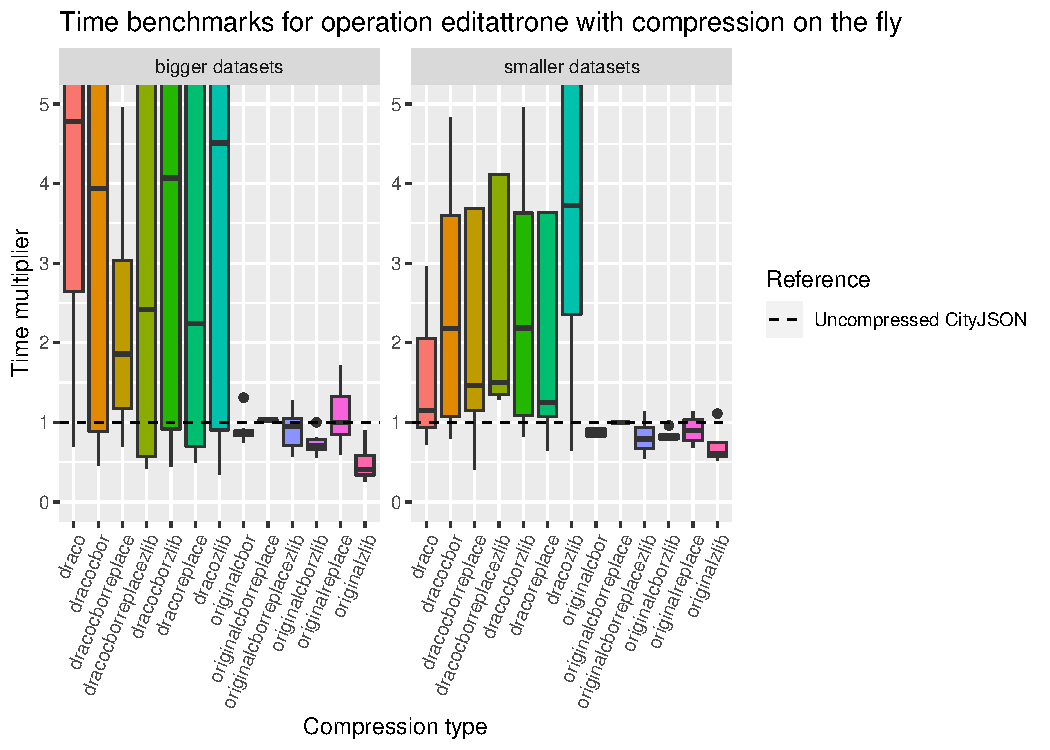
\includegraphics[scale=0.92]{figs/benchmark/individualotf/editattrone.pdf}
    \caption{Boxplots of time performance of (on the fly) compressed datasets on editing attributes of one feature compared to uncompressed CityJSON.}
    \label{figotf:sdvis}
\end{figure}

The data is edited before being compressed with this use case.
Draco is again not suitable to use when compressing data on the fly with neither large nor small datasets.
As for the other compression types, original-zlib and original-cbor-zlib are beneficial for performance with the larger ones, but with the smaller ones only original-cbor and original-cbor-zlib have a (slight) advantage in every case.
The box plots of the other types stretch above the baseline.

On the fly compression can improve the attribute editing time of CityJSON datasets on one city object to 33\% or 60\% (when respectively using large datasets and small datasets) of the time that it takes to perform the same operation with uncompressed CityJSON.



\begin{table}[!h]
    \begin{minipage}{.5\linewidth}
      \caption{
Median performance with editattrone on large datasets, compression on the fly}
\centering

\begin{tabular}{|l|r|}
\hline
Compression type & median\\
\hline
originalzlib & 0.330\\
\hline
dracocborreplacezlib & 0.420\\
\hline
originalcborzlib & 0.570\\
\hline
dracoreplace & 0.760\\
\hline
originalcbor & 0.870\\
\hline
originalcborreplacezlib & 0.960\\
\hline
originalreplace & 1.075\\
\hline
dracocbor & 4.600\\
\hline
dracozlib & 4.990\\
\hline
draco & 5.480\\
\hline
dracocborzlib & 5.610\\
\hline
\end{tabular}
\end{minipage}%
    \begin{minipage}{.5\linewidth}
      \centering
        \caption{
Median performance with editattrone on small datasets, compression on the fly}

\begin{tabular}{|l|r|}
\hline
Compression type & median\\
\hline
originalzlib & 0.605\\
\hline
originalcborreplacezlib & 0.790\\
\hline
originalcborzlib & 0.800\\
\hline
originalcbor & 0.870\\
\hline
originalreplace & 0.900\\
\hline
originalcborreplace & 1.000\\
\hline
draco & 1.150\\
\hline
dracoreplace & 1.250\\
\hline
dracocborreplace & 1.460\\
\hline
dracocborreplacezlib & 1.500\\
\hline
dracocbor & 2.180\\
\hline
dracocborzlib & 2.185\\
\hline
dracozlib & 3.725\\
\hline
\end{tabular}
\end{minipage} 
\end{table}

\newpage


\subsection{Editing attributes all features}

\subsubsection{Compression in advance}

\begin{figure}[h!]
    %\hspace*{-2.3cm}  
    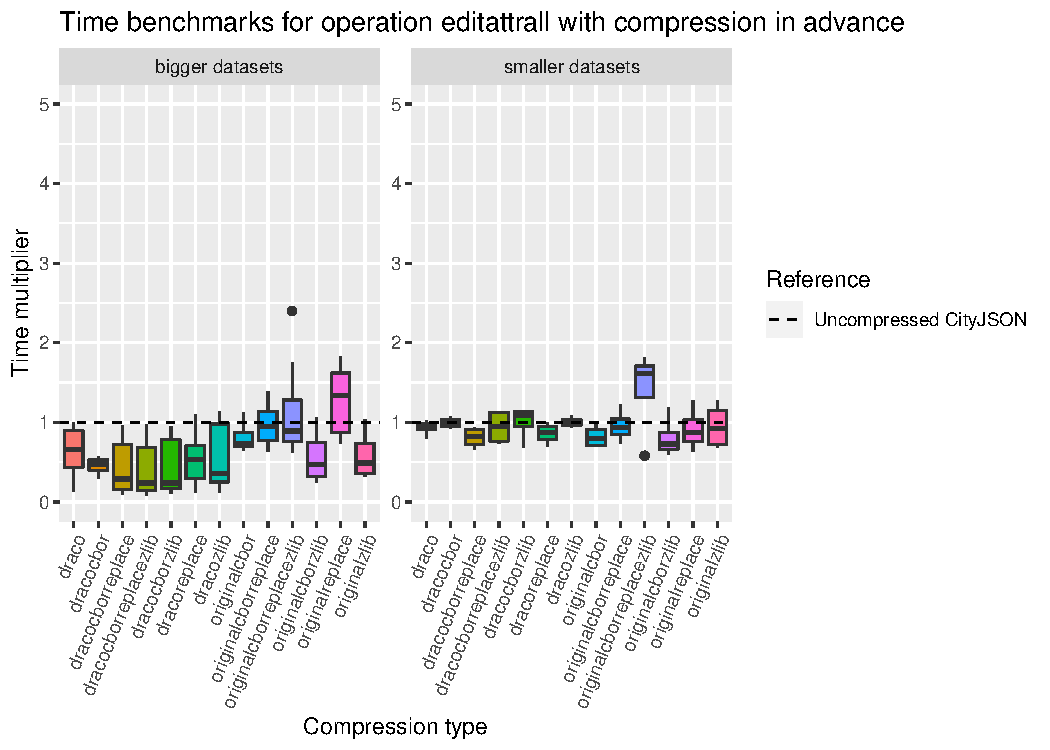
\includegraphics[scale=0.92]{figs/benchmark/individual/editattrall.pdf}
    \caption{Boxplots of time performance of (in advance) compressed datasets on editing attributes of all features compared to uncompressed CityJSON.}
    \label{fig:sdvis}
\end{figure}

When editing the attributes of a large dataset it is not a good idea to use the replace method, regardless of the seemingly more efficient way to edit attributes with it (see Section~\ref{sec:impleditone}).
But apart from that, compression is beneficial for this use case.
Using Draco works well, which would be because it is untouched as only attributes are edited and Draco geometries are small, benefitting the transmission time.
Original-cbor, original-cbor-zlib, and original-zlib also perform well.

With the small datasets most compression types do not always perform well---only draco-cbor-replace has a boxplot that remains under the baseline.
This means that the overhead when compressing the data again does not outweigh the benefits of compression as much as with large datasets.

Compression in advance can improve the attribute editing time of CityJSON datasets on all city objects to 14\% or 72\% (when respectively using large datasets and small datasets) of the time that it takes to perform the same operation with uncompressed CityJSON.


  \begin{table}[!h]
    \begin{minipage}{.5\linewidth}
      \caption{
Median performance with editattrall on large datasets, compression in advance}
\centering

\begin{tabular}{|l|r|}
\hline
Compression type & median\\
\hline
dracocborreplace & 0.140\\
\hline
dracocborreplacezlib & 0.170\\
\hline
dracocborzlib & 0.205\\
\hline
originalcborzlib & 0.300\\
\hline
dracozlib & 0.350\\
\hline
originalzlib & 0.355\\
\hline
dracoreplace & 0.410\\
\hline
dracocbor & 0.475\\
\hline
draco & 0.630\\
\hline
originalcbor & 0.715\\
\hline
originalcborreplace & 1.130\\
\hline
originalreplace & 1.490\\
\hline
originalcborreplacezlib & 1.510\\
\hline
\end{tabular}
\end{minipage}%
    \begin{minipage}{.5\linewidth}
      \centering
        \caption{
Median performance with editattrall on small datasets, compression in advance}

\begin{tabular}{|l|r|}
\hline
Compression type & median\\
\hline
originalcborzlib & 0.725\\
\hline
originalcbor & 0.795\\
\hline
dracocborreplace & 0.820\\
\hline
dracoreplace & 0.870\\
\hline
originalreplace & 0.875\\
\hline
originalzlib & 0.925\\
\hline
originalcborreplace & 0.935\\
\hline
dracocborreplacezlib & 0.945\\
\hline
draco & 0.965\\
\hline
dracocbor & 0.995\\
\hline
dracozlib & 0.995\\
\hline
dracocborzlib & 1.090\\
\hline
originalcborreplacezlib & 1.615\\
\hline
\end{tabular}
\end{minipage} 
\end{table}

\clearpage

\subsubsection{Compression on the fly}

\begin{figure}[h!]
    %\hspace*{-2.3cm}  
    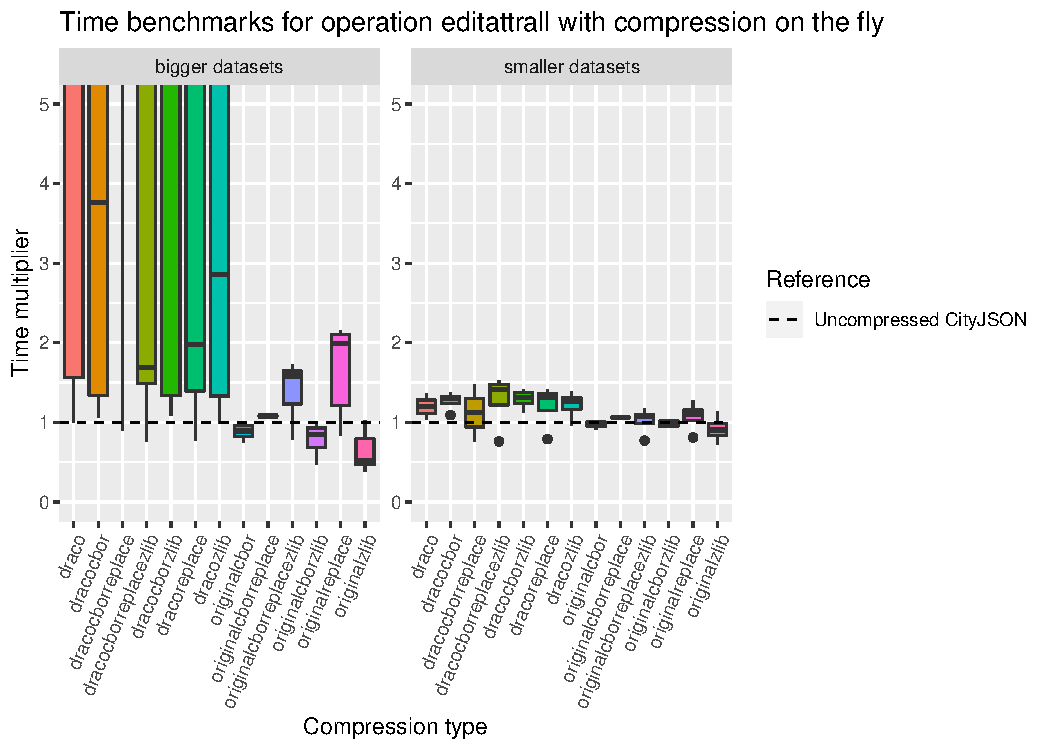
\includegraphics[scale=0.92]{figs/benchmark/individualotf/editattrall.pdf}
    \caption{Boxplots of time performance of (on the fly) compressed datasets on editing attributes of all features compared to uncompressed CityJSON.}
    \label{figotf:sdvis}
\end{figure}


As is always the case with compression on the fly, the use of Draco compression is detrimental for performance.
With the large datasets original-cbor, original-cbor-zlib, and original-zlib yield a proper performance gain, which would be the result of a good balance between file size and (de)compression time.
As for the small datasets, the differences between the compression types are smaller and there is no clear best one to use as the better performing ones are around the baseline.
Thus in that case you might be better off not using compression at all.


On the fly compression can improve the attribute editing time of CityJSON datasets on all city objects to 47\% or 90\% (when respectively using large datasets and small datasets) of the time that it takes to perform the same operation with uncompressed CityJSON.



  \begin{table}[!h]
    \begin{minipage}{.5\linewidth}
      \caption{
Median performance with editattrall on large datasets, compression on the fly}
\centering

\begin{tabular}{|l|r|}
\hline
Compression type & median\\
\hline
originalzlib & 0.475\\
\hline
originalcborzlib & 0.680\\
\hline
originalcbor & 0.825\\
\hline
originalcborreplacezlib & 1.660\\
\hline
originalreplace & 2.105\\
\hline
dracoreplace & 15.180\\
\hline
dracozlib & 16.910\\
\hline
dracocborreplacezlib & 16.950\\
\hline
draco & 18.210\\
\hline
dracocborreplace & 27.220\\
\hline
dracocborzlib & 28.735\\
\hline
dracocbor & 32.745\\
\hline
\end{tabular}
\end{minipage}%
    \begin{minipage}{.5\linewidth}
      \centering
        \caption{
Median performance with editattrall on small datasets, compression on the fly}

\begin{tabular}{|l|r|}
\hline
Compression type & median\\
\hline
originalzlib & 0.905\\
\hline
originalcbor & 0.980\\
\hline
originalcborzlib & 0.980\\
\hline
originalcborreplace & 1.060\\
\hline
originalcborreplacezlib & 1.070\\
\hline
originalreplace & 1.105\\
\hline
dracocborreplace & 1.120\\
\hline
draco & 1.200\\
\hline
dracozlib & 1.260\\
\hline
dracocbor & 1.300\\
\hline
dracoreplace & 1.310\\
\hline
dracocborzlib & 1.315\\
\hline
dracocborreplacezlib & 1.415\\
\hline
\end{tabular}
\end{minipage} 
\end{table}

\clearpage

\section{Editing (geometry)}
\label{bmeditinggeom}

\subsection{Editing geometry one feature}
\label{sec:bmeditone}

\subsubsection{Compression in advance}


\begin{figure}[h!]
    %\hspace*{-2.3cm}  
    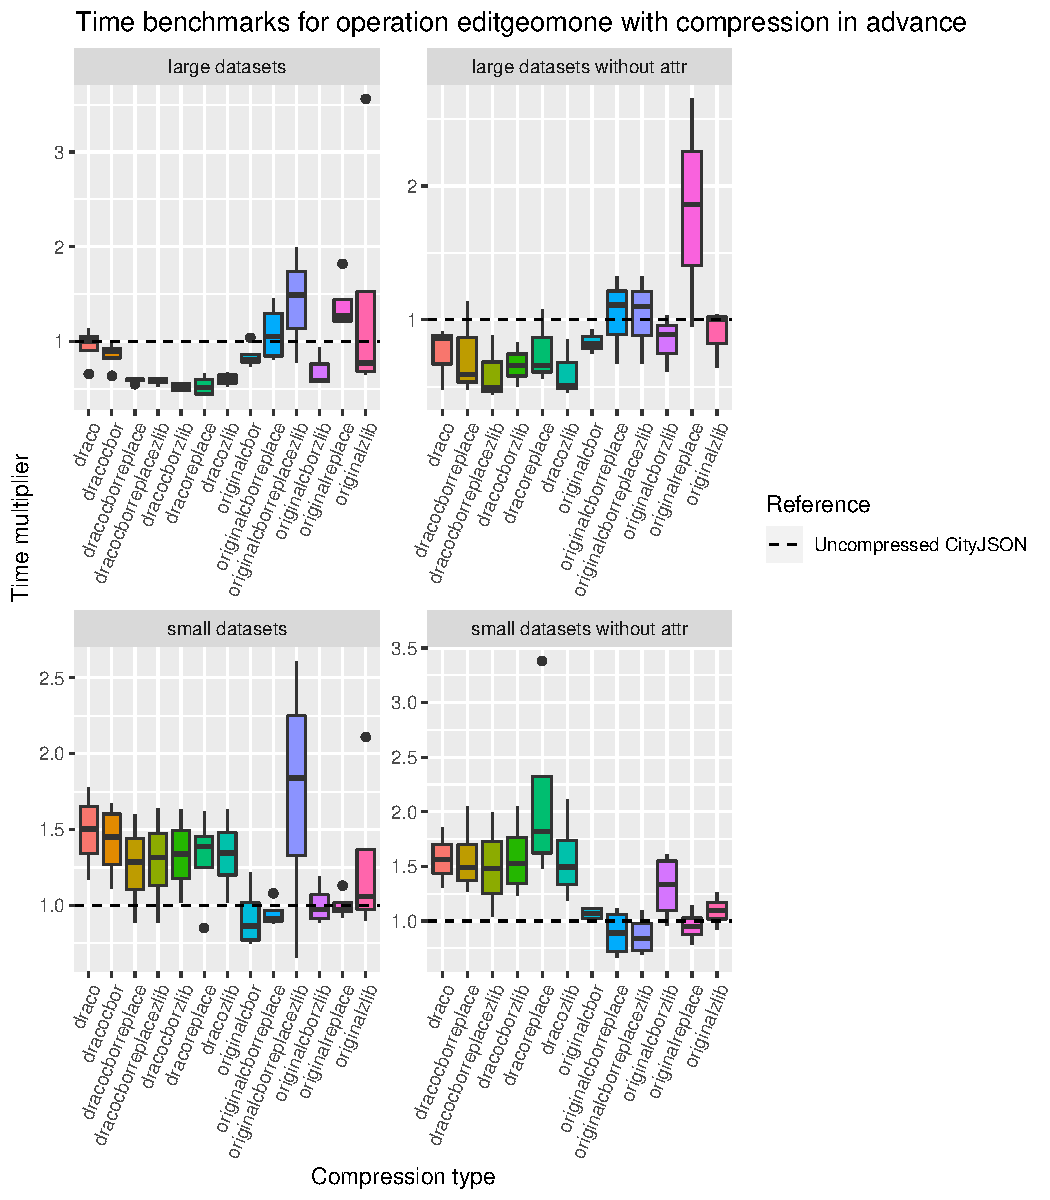
\includegraphics[scale=0.92]{figs/benchmark/individual/editgeomone.pdf}
    \caption{Boxplots of time performance of (in advance) compressed datasets on editing geometry of one feature compared to uncompressed CityJSON.}
    \label{fig:sdvis}
\end{figure}

Draco is suitable for this use case when editing large datasets.
This is despite Draco methods having high compression times as shown in Section~\ref{sec:encodingperformance}.
But the results in that Section were created by compressing CityJSON geometries into Draco geometries with OBJ conversion as intermediate step (see Section~\ref{sec:dracocompressiontypes}).
In this case however the Draco geometries are edited directly as they are decoded in the client.
It can then be compressed again without additional steps.
The use of additional compression techniques is beneficial as well.
If not using Draco, original-cbor and original-cbor-zlib are good choices.
This is the same for datasets that do not contain attributes.

With the small datasets none of the compression types perform particularly well.
Draco is now not beneficial which would be due to the overhead of Draco compression that is more significant with small data.
Original-cbor has the lowest median with attributes, but is above the baseline with datasets that do not have attributes.
In that case there is less data for \ac{cbor} to compress which could be the explaining factor.

Compression in advance can improve the geometry editing time of CityJSON datasets on one city object to 51\%, 49\%, 86\%, or 84\% (when respectively using large datasets, large datasets without attributes, small datasets, and small datasets without attributes) of the time that it takes to perform the same operation with uncompressed CityJSON.



  \begin{table}[!h]
    \begin{minipage}{.5\linewidth}
      \caption{
Median performance with editgeomone on large datasets, compression in advance}
\centering

\begin{tabular}{|l|r|}
\hline
Compression type & median\\
\hline
dracoreplace & 0.515\\
\hline
dracocborzlib & 0.520\\
\hline
originalcborzlib & 0.590\\
\hline
dracocborreplacezlib & 0.595\\
\hline
dracocborreplace & 0.600\\
\hline
dracozlib & 0.605\\
\hline
originalzlib & 0.775\\
\hline
originalcbor & 0.805\\
\hline
dracocbor & 0.895\\
\hline
draco & 1.005\\
\hline
originalcborreplace & 1.055\\
\hline
originalreplace & 1.270\\
\hline
originalcborreplacezlib & 1.490\\
\hline
\end{tabular}
\end{minipage}%
    \begin{minipage}{.5\linewidth}
      \centering
        \caption{
Median performance with editgeomone on large datasets without attributes, compression in advance}

\begin{tabular}{|l|r|}
\hline
Compression type & median\\
\hline
dracocborreplacezlib & 0.49\\
\hline
dracozlib & 0.51\\
\hline
dracocborreplace & 0.59\\
\hline
dracocborzlib & 0.66\\
\hline
dracoreplace & 0.66\\
\hline
originalcbor & 0.82\\
\hline
draco & 0.86\\
\hline
originalcborzlib & 0.89\\
\hline
originalzlib & 1.00\\
\hline
originalcborreplacezlib & 1.10\\
\hline
originalcborreplace & 1.11\\
\hline
originalreplace & 1.86\\
\hline
\end{tabular}
\end{minipage} 
\end{table}
\begin{table}[!h]
    \begin{minipage}{.5\linewidth}
      \caption{
Median performance with editgeomone on small datasets, compression in advance}
\centering

\begin{tabular}{|l|r|}
\hline
Compression type & median\\
\hline
originalcbor & 0.865\\
\hline
originalcborreplace & 0.915\\
\hline
originalreplace & 0.975\\
\hline
originalcborzlib & 0.975\\
\hline
originalzlib & 1.060\\
\hline
dracocborreplace & 1.285\\
\hline
dracocborreplacezlib & 1.315\\
\hline
dracocborzlib & 1.340\\
\hline
dracozlib & 1.345\\
\hline
dracoreplace & 1.390\\
\hline
dracocbor & 1.450\\
\hline
draco & 1.505\\
\hline
originalcborreplacezlib & 1.840\\
\hline
\end{tabular}
\end{minipage}%
    \begin{minipage}{.5\linewidth}
      \centering
        \caption{
Median performance with editgeomone on small datasets without attributes, compression in advance}

\begin{tabular}{|l|r|}
\hline
Compression type & median\\
\hline
originalcborreplacezlib & 0.840\\
\hline
originalcborreplace & 0.890\\
\hline
originalreplace & 0.950\\
\hline
originalcbor & 1.070\\
\hline
originalzlib & 1.095\\
\hline
originalcborzlib & 1.335\\
\hline
dracocborreplacezlib & 1.480\\
\hline
dracocborreplace & 1.490\\
\hline
dracozlib & 1.495\\
\hline
dracocborzlib & 1.525\\
\hline
draco & 1.565\\
\hline
dracoreplace & 1.820\\
\hline
\end{tabular}
\end{minipage} 
\end{table}

\clearpage

\subsubsection{Compression on the fly}

\begin{figure}[h!]
    %\hspace*{-2.3cm}  
    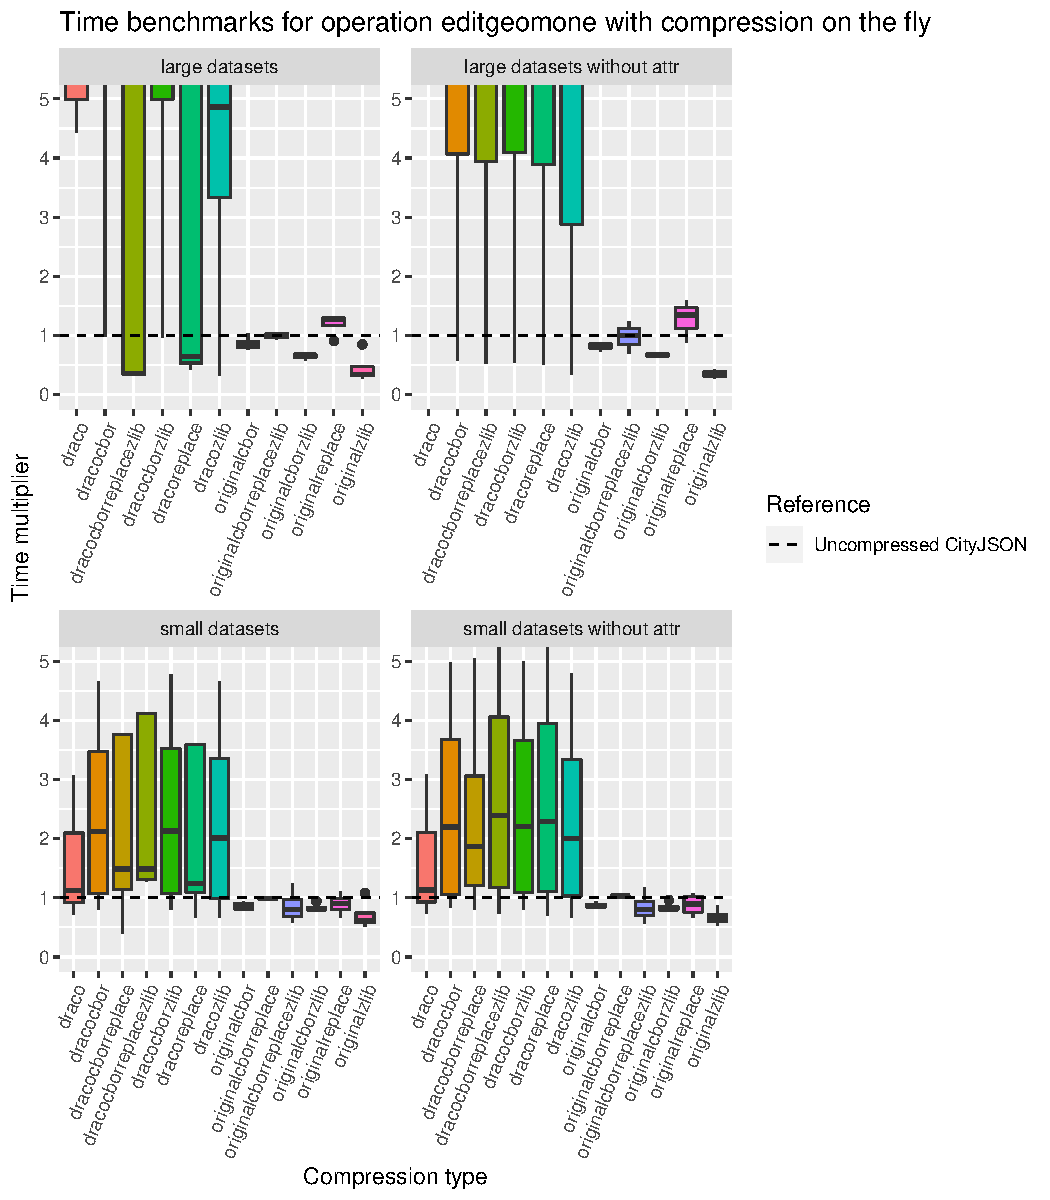
\includegraphics[scale=0.92]{figs/benchmark/individualotf/editgeomone.pdf}
    \caption{Boxplots of time performance of (on the fly) compressed datasets on editing geometry of one feature compared to uncompressed CityJSON.}
    \label{figotf:sdvis}
\end{figure}

Ignoring the compression types using Draco, it can be beneficial to use compression on the fly for this use case.
With large datasets, original-cbor, original-zlib, and original-cbor-zlib do well.
They are also fine to use with small datasets, but here the compression types have similar performances.
There are no other notable observations to be made.

On the fly compression can improve the geometry editing time of CityJSON datasets on one city object to 34\%, 36\%, 61\%, or 64\% (when respectively using large datasets, large datasets without attributes, small datasets, and small datasets without attributes) of the time that it takes to perform the same operation with uncompressed CityJSON.



  \begin{table}[!h]
    \begin{minipage}{.5\linewidth}
      \caption{
Median performance with editgeomone on large datasets, compression on the fly}
\centering

\begin{tabular}{|l|r|}
\hline
Compression type & median\\
\hline
originalzlib & 0.345\\
\hline
dracocborreplacezlib & 0.360\\
\hline
dracoreplace & 0.650\\
\hline
originalcborzlib & 0.680\\
\hline
originalcbor & 0.830\\
\hline
originalcborreplacezlib & 1.000\\
\hline
originalreplace & 1.270\\
\hline
dracozlib & 4.860\\
\hline
draco & 5.540\\
\hline
dracocborzlib & 9.020\\
\hline
dracocbor & 11.700\\
\hline
\end{tabular}
\end{minipage}%
    \begin{minipage}{.5\linewidth}
      \centering
        \caption{
Median performance with editgeomone on large datasets without attributes, compression on the fly}

\begin{tabular}{|l|r|}
\hline
Compression type & median\\
\hline
originalzlib & 0.36\\
\hline
originalcborzlib & 0.66\\
\hline
originalcbor & 0.85\\
\hline
originalcborreplacezlib & 1.00\\
\hline
originalreplace & 1.35\\
\hline
dracozlib & 5.42\\
\hline
draco & 6.60\\
\hline
dracoreplace & 7.26\\
\hline
dracocborreplacezlib & 7.37\\
\hline
dracocbor & 7.56\\
\hline
dracocborzlib & 7.63\\
\hline
\end{tabular}
\end{minipage} 
\end{table}
\begin{table}[!h]
    \begin{minipage}{.5\linewidth}
      \caption{
Median performance with editgeomone on small datasets, compression on the fly}
\centering

\begin{tabular}{|l|r|}
\hline
Compression type & median\\
\hline
originalzlib & 0.615\\
\hline
originalcborreplacezlib & 0.800\\
\hline
originalcborzlib & 0.805\\
\hline
originalcbor & 0.855\\
\hline
originalreplace & 0.900\\
\hline
originalcborreplace & 0.990\\
\hline
draco & 1.120\\
\hline
dracoreplace & 1.240\\
\hline
dracocborreplacezlib & 1.485\\
\hline
dracocborreplace & 1.490\\
\hline
dracozlib & 2.010\\
\hline
dracocbor & 2.120\\
\hline
dracocborzlib & 2.130\\
\hline
\end{tabular}
\end{minipage}%
    \begin{minipage}{.5\linewidth}
      \centering
        \caption{
Median performance with editgeomone on small datasets without attributes, compression on the fly}

\begin{tabular}{|l|r|}
\hline
Compression type & median\\
\hline
originalzlib & 0.640\\
\hline
originalcborreplacezlib & 0.805\\
\hline
originalcborzlib & 0.815\\
\hline
originalcbor & 0.865\\
\hline
originalreplace & 0.895\\
\hline
originalcborreplace & 1.030\\
\hline
draco & 1.130\\
\hline
dracocborreplace & 1.870\\
\hline
dracozlib & 2.000\\
\hline
dracocbor & 2.195\\
\hline
dracocborzlib & 2.205\\
\hline
dracoreplace & 2.290\\
\hline
dracocborreplacezlib & 2.390\\
\hline
\end{tabular}
\end{minipage} 
\end{table}

\newpage

\subsection{Editing geometry all features}


\subsubsection{Compression in advance}

\begin{figure}[h!]
    %\hspace*{-2.3cm}  
    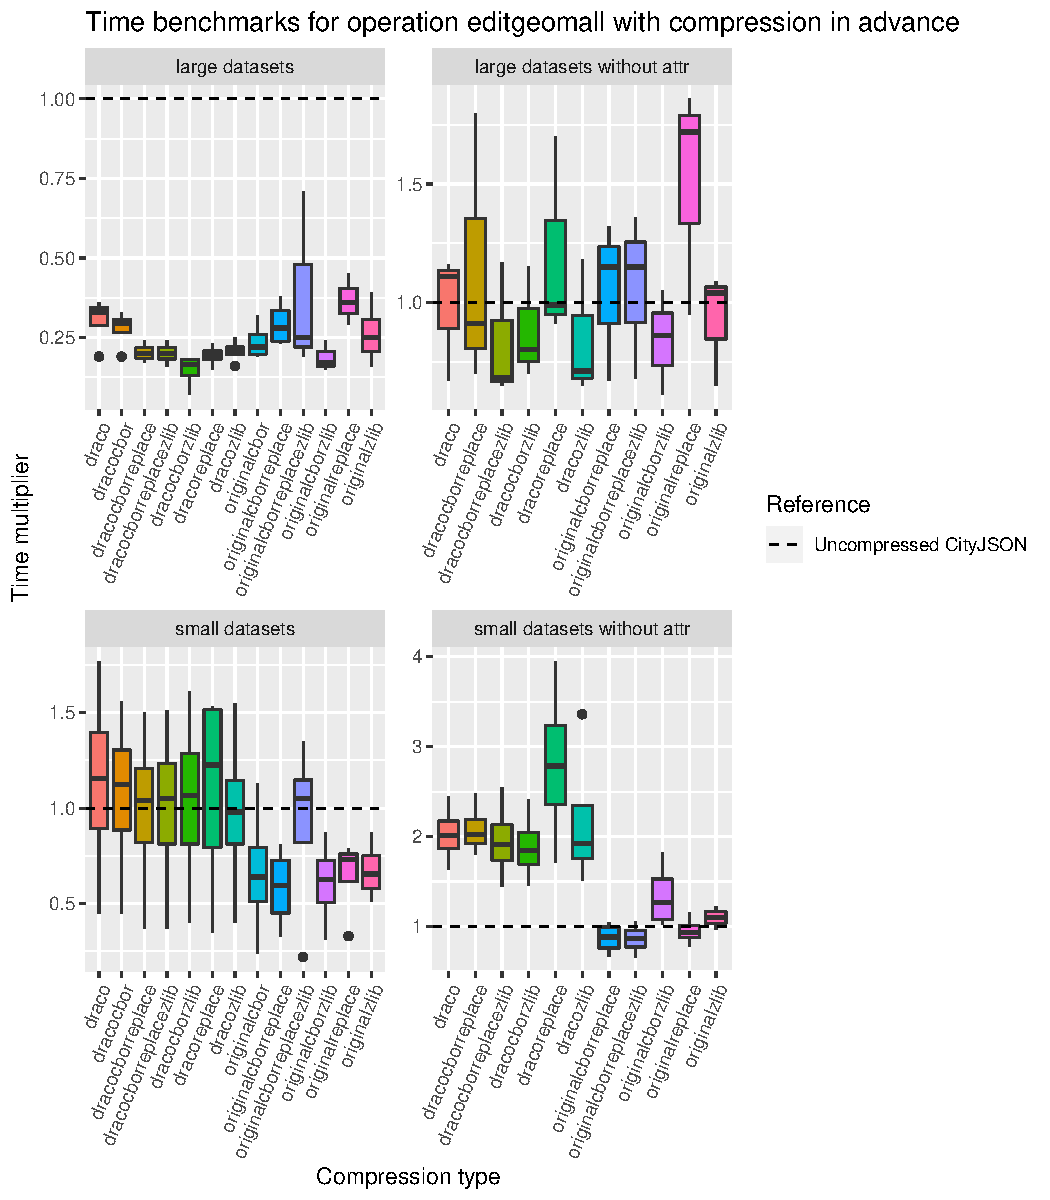
\includegraphics[scale=0.92]{figs/benchmark/individual/editgeomall.pdf}
    \caption{Boxplots of time performance of (in advance) compressed datasets on editing geometry of all features compared to uncompressed CityJSON.}
    \label{fig:sdvis}
\end{figure}

With the large datasets that include attributes all compression types perform well.
This is not seen when only editing the geometry of one city object, when performance was only good with Draco.
It is surprising because now all city objects have to be traversed for compression types without Draco, but with Draco all vertices already had to be iterated over, even when just wanting to edit one feature (see Section~\ref{sec:impleditgeomone}).
The results are also quite different for large datasets without attributes, and generally worse---none of the compression types is good to use with every of these datasets as the boxplots indicate.
This is surprising as well since there is less data to compress again after the editing in that case.

As for the small datasets, Draco compresses negatively influences the performance, presumably because of the overhead.
Other compression types generally work well, except for draco-cbor-replace-zlib when attributes are included and original-cbor-zlib when they are not.
The latter one tends to perform well in other use cases so it could be an anomaly.
The former type includes the replace method that does not do well so far, but other compression types that use it do not do as bad.
This can indicate that it is not worth it to compress the array of attributes with zlib (see Section~\ref{sec:implreplace}).

Compression in advance can improve the geometry editing time of CityJSON datasets on all city objects to 16\%, 68\%, 59\%, or 86\% (when respectively using large datasets, large datasets without attributes, small datasets, and small datasets without attributes) of the time that it takes to perform the same operation with uncompressed CityJSON.


  \begin{table}[!h]
    \begin{minipage}{.5\linewidth}
      \caption{
Median performance with editgeomall on large datasets, compression in advance}
\centering

\begin{tabular}{|l|r|}
\hline
Compression type & median\\
\hline
dracocborzlib & 0.165\\
\hline
originalcborzlib & 0.170\\
\hline
dracoreplace & 0.195\\
\hline
dracocborreplace & 0.200\\
\hline
dracocborreplacezlib & 0.200\\
\hline
dracozlib & 0.210\\
\hline
originalcbor & 0.220\\
\hline
originalcborreplacezlib & 0.250\\
\hline
originalzlib & 0.250\\
\hline
originalcborreplace & 0.280\\
\hline
dracocbor & 0.295\\
\hline
draco & 0.330\\
\hline
originalreplace & 0.360\\
\hline
\end{tabular}
\end{minipage}%
    \begin{minipage}{.5\linewidth}
      \centering
        \caption{
Median performance with editgeomall on large datasets without attributes, compression in advance}

\begin{tabular}{|l|r|}
\hline
Compression type & median\\
\hline
dracocborreplacezlib & 0.68\\
\hline
dracozlib & 0.71\\
\hline
dracocborzlib & 0.80\\
\hline
originalcborzlib & 0.86\\
\hline
dracocborreplace & 0.91\\
\hline
dracoreplace & 0.99\\
\hline
originalzlib & 1.04\\
\hline
draco & 1.11\\
\hline
originalcborreplace & 1.15\\
\hline
originalcborreplacezlib & 1.15\\
\hline
originalreplace & 1.72\\
\hline
\end{tabular}
\end{minipage} 
\end{table}
\begin{table}[!h]
    \begin{minipage}{.5\linewidth}
      \caption{
Median performance with editgeomall on small datasets, compression in advance}
\centering

\begin{tabular}{|l|r|}
\hline
Compression type & median\\
\hline
originalcborreplace & 0.595\\
\hline
originalcborzlib & 0.625\\
\hline
originalcbor & 0.640\\
\hline
originalzlib & 0.655\\
\hline
originalreplace & 0.730\\
\hline
dracozlib & 0.980\\
\hline
dracocborreplace & 1.040\\
\hline
dracocborreplacezlib & 1.050\\
\hline
originalcborreplacezlib & 1.050\\
\hline
dracocborzlib & 1.065\\
\hline
dracocbor & 1.125\\
\hline
draco & 1.155\\
\hline
dracoreplace & 1.225\\
\hline
\end{tabular}
\end{minipage}%
    \begin{minipage}{.5\linewidth}
      \centering
        \caption{
Median performance with editgeomall on small datasets without attributes, compression in advance}

\begin{tabular}{|l|r|}
\hline
Compression type & median\\
\hline
originalcborreplacezlib & 0.865\\
\hline
originalcborreplace & 0.885\\
\hline
originalreplace & 0.935\\
\hline
originalzlib & 1.100\\
\hline
originalcborzlib & 1.265\\
\hline
dracocborzlib & 1.845\\
\hline
dracocborreplacezlib & 1.910\\
\hline
dracozlib & 1.925\\
\hline
draco & 2.010\\
\hline
dracocborreplace & 2.025\\
\hline
dracoreplace & 2.785\\
\hline
\end{tabular}
\end{minipage} 
\end{table}

\clearpage

\subsubsection{Compression on the fly}

\begin{figure}[h!]
    %\hspace*{-2.3cm}  
    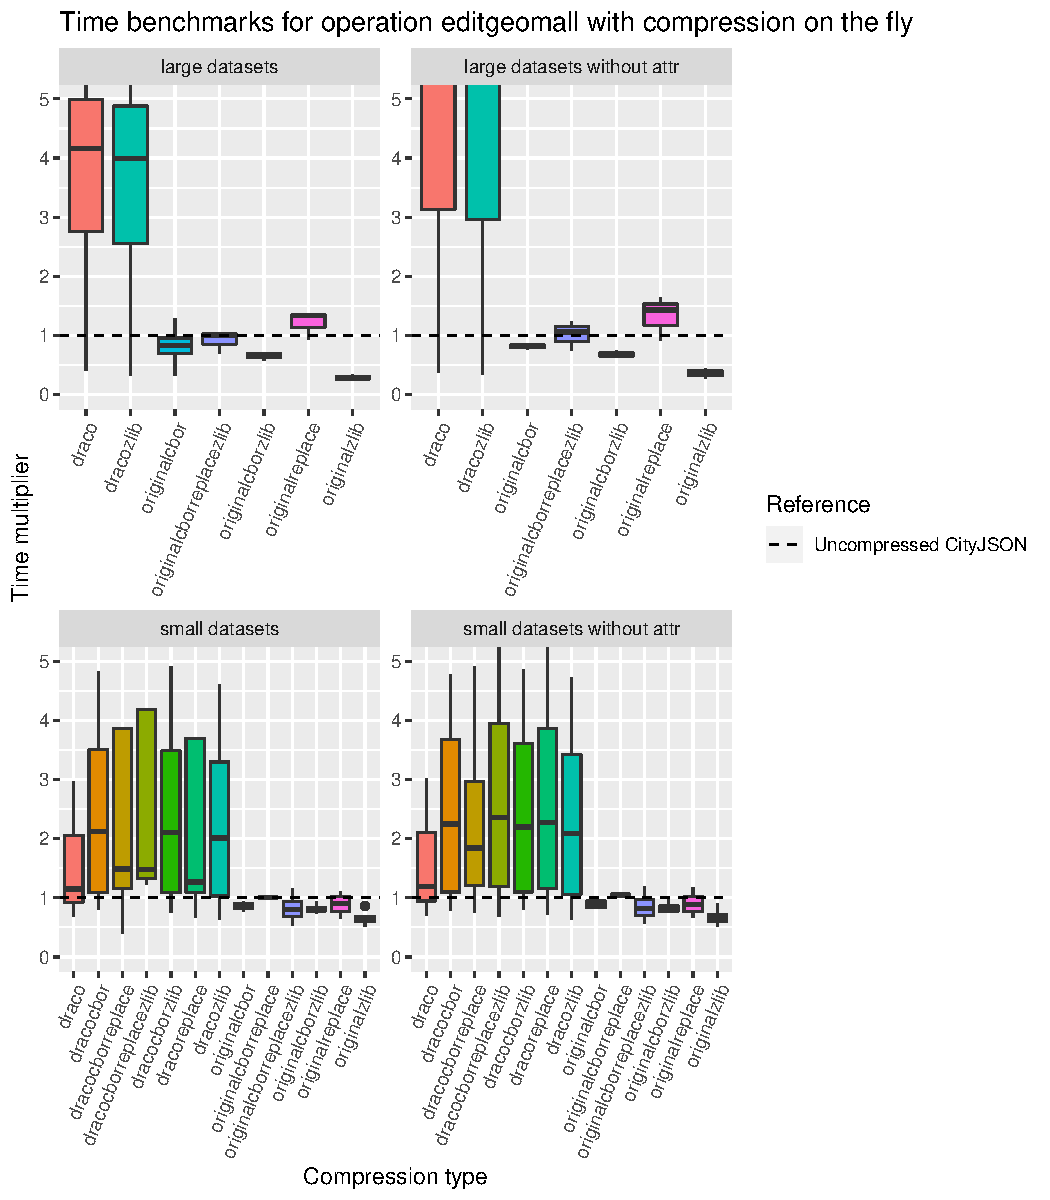
\includegraphics[scale=0.92]{figs/benchmark/individualotf/editgeomall.pdf}
    \caption{Boxplots of time performance of (on the fly) compressed datasets on editing geometry of all features compared to uncompressed CityJSON.}
    \label{figotf:sdvis}
\end{figure}

There was an error with multiple compression types in combination with this use case and large datasets, which is why they are missing from the charts.
It is not very important, since it was mostly a problem with Draco which has already proven to perform badly with on the fly compression.

What happens in this use case is that basically full datasets are compressed after all being edited with the same algorithm.
The results are thus not so interesting and should come close to the theoretical perormance gain.
With the large datasets original-zlib and original-cbor-zlib do well, and original-cbor as well when attributes are not included.
As for the small datasets, these three do well with both small dataset types.
They are relatively uncomplicated compression types and their good performance can be explained by the balance between file size and processing time, despite compression time being included.

On the fly compression can improve the geometry editing time of CityJSON datasets on all city objects to 28\%, 37\%, 62\%, or 64\% (when respectively using large datasets, large datasets without attributes, small datasets, and small datasets without attributes) of the time that it takes to perform the same operation with uncompressed CityJSON.


\begin{table}[!h]
    \begin{minipage}{.5\linewidth}
      \caption{
Median performance with editgeomall on large datasets, compression on the fly}
\centering

\begin{tabular}{|l|r|}
\hline
Compression type & median\\
\hline
originalzlib & 0.280\\
\hline
originalcborzlib & 0.680\\
\hline
originalcbor & 0.835\\
\hline
originalcborreplacezlib & 1.010\\
\hline
originalreplace & 1.340\\
\hline
dracozlib & 3.995\\
\hline
draco & 4.165\\
\hline
\end{tabular}
\end{minipage}%
    \begin{minipage}{.5\linewidth}
      \centering
        \caption{
Median performance with editgeomall on large datasets without attributes, compression on the fly}

\begin{tabular}{|l|r|}
\hline
Compression type & median\\
\hline
originalzlib & 0.37\\
\hline
originalcborzlib & 0.66\\
\hline
originalcbor & 0.83\\
\hline
originalcborreplacezlib & 1.06\\
\hline
originalreplace & 1.43\\
\hline
dracozlib & 5.58\\
\hline
draco & 5.89\\
\hline
\end{tabular}
\end{minipage} 
\end{table}
\begin{table}[!h]
    \begin{minipage}{.5\linewidth}
      \caption{
Median performance with editgeomall on small datasets, compression on the fly}
\centering

\begin{tabular}{|l|r|}
\hline
Compression type & median\\
\hline
originalzlib & 0.625\\
\hline
originalcborreplacezlib & 0.800\\
\hline
originalcborzlib & 0.800\\
\hline
originalcbor & 0.870\\
\hline
originalreplace & 0.905\\
\hline
originalcborreplace & 1.010\\
\hline
draco & 1.150\\
\hline
dracoreplace & 1.265\\
\hline
dracocborreplacezlib & 1.480\\
\hline
dracocborreplace & 1.485\\
\hline
dracozlib & 2.010\\
\hline
dracocborzlib & 2.105\\
\hline
dracocbor & 2.125\\
\hline
\end{tabular}
\end{minipage}%
    \begin{minipage}{.5\linewidth}
      \centering
        \caption{
Median performance with editgeomall on small datasets without attributes, compression on the fly}

\begin{tabular}{|l|r|}
\hline
Compression type & median\\
\hline
originalzlib & 0.640\\
\hline
originalcborzlib & 0.800\\
\hline
originalcborreplacezlib & 0.820\\
\hline
originalreplace & 0.885\\
\hline
originalcbor & 0.890\\
\hline
originalcborreplace & 1.050\\
\hline
draco & 1.190\\
\hline
dracocborreplace & 1.840\\
\hline
dracozlib & 2.090\\
\hline
dracocborzlib & 2.195\\
\hline
dracocbor & 2.250\\
\hline
dracoreplace & 2.275\\
\hline
dracocborreplacezlib & 2.355\\
\hline
\end{tabular}
\end{minipage} 
\end{table}



\newpage
\section{Conclusion and recommendations}
\label{bmconclusion}

\begin{figure}[h!]
    %\hspace*{-2.3cm}  
    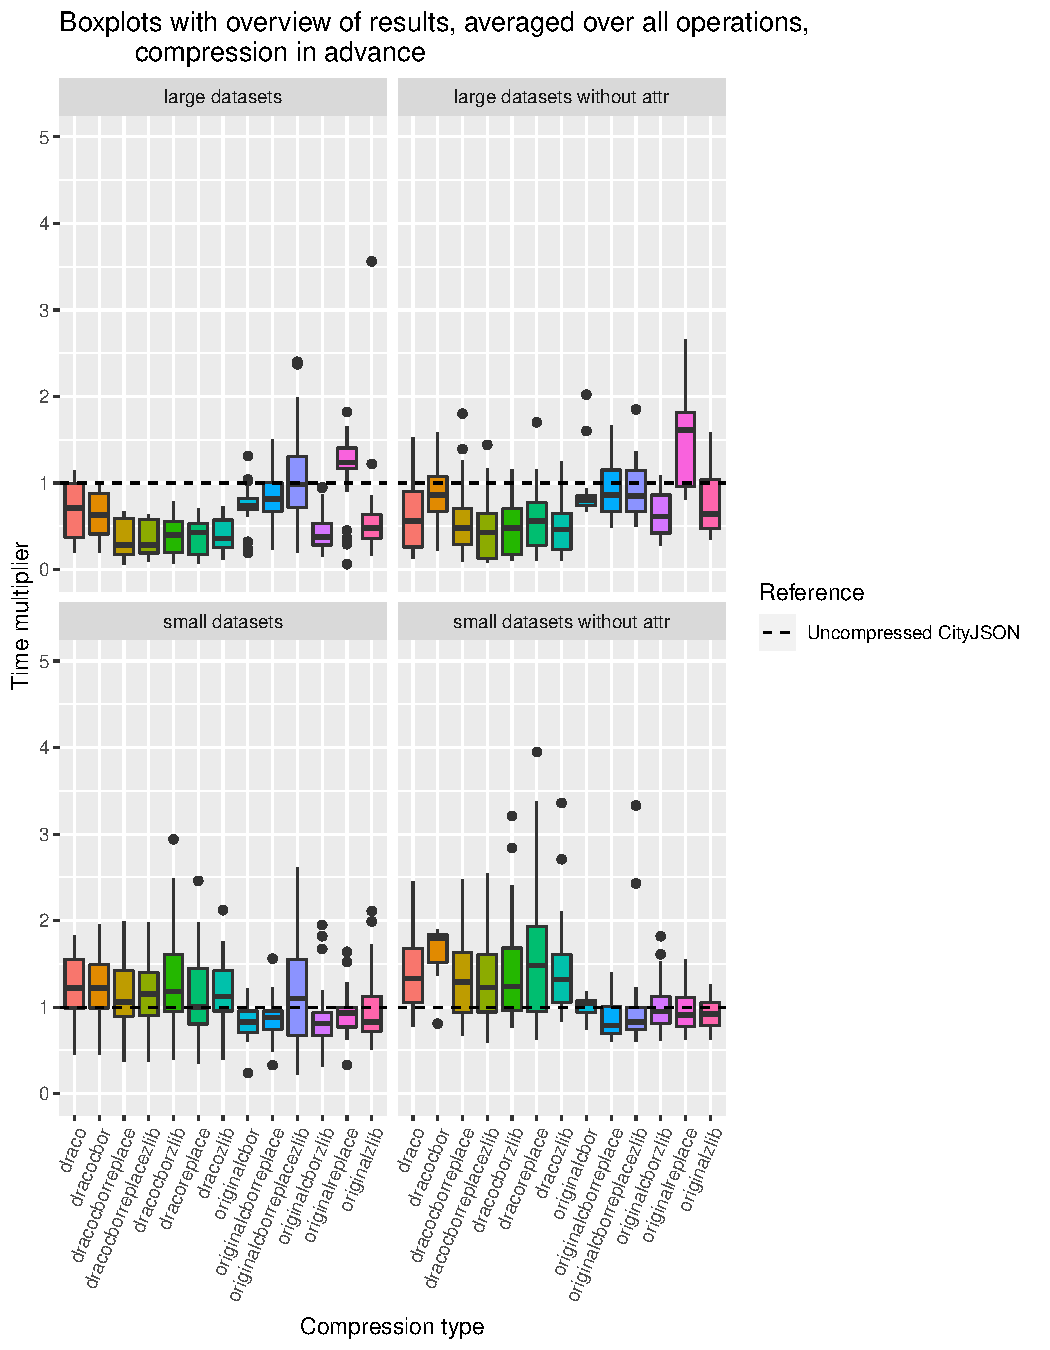
\includegraphics[scale=0.92]{figs/benchmark/overview/fulloverviewia.pdf}
    \caption{Overview of the performance of all compression types by dataset type. The results are averaged over every operation.}
    \label{fig:performanceoverview}
\end{figure}

\begin{figure}[h!]
    %\hspace*{-2.3cm}  
    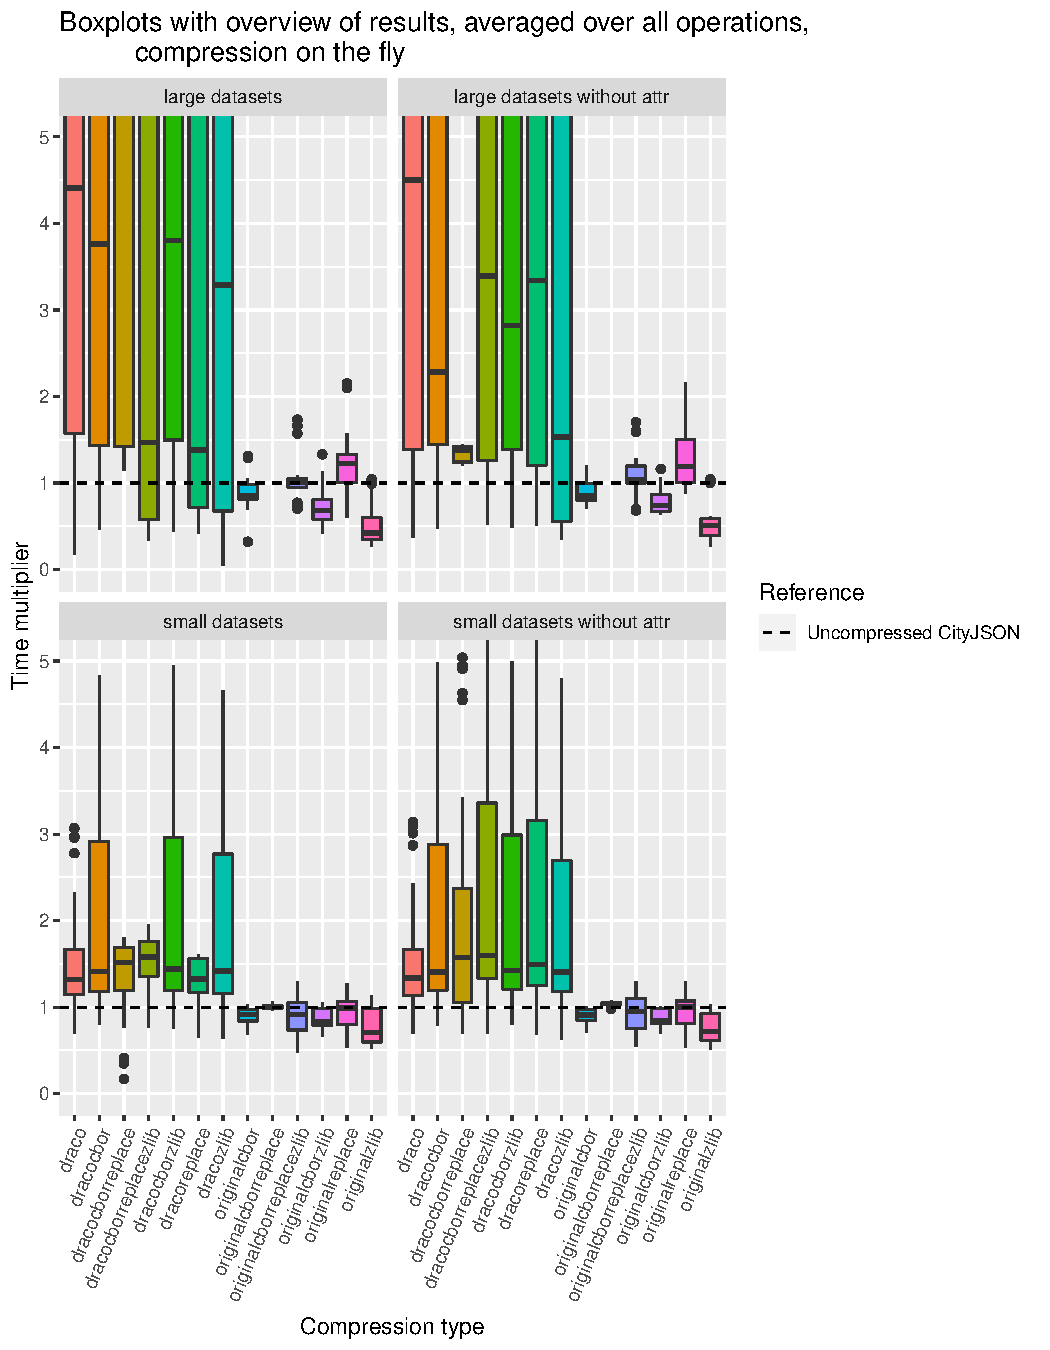
\includegraphics[scale=0.92]{figs/benchmark/overview/fulloverviewotf.pdf}
    \caption{Overview of the performance of all compression types by dataset type. The results are averaged over every operation.}
    \label{fig:performanceoverviewotf}
\end{figure}

\clearpage


On Figures~\ref{fig:performanceoverview} and ~\ref{fig:performanceoverviewotf}, the difference between operations is removed here such that appropriate compression types for general purpose can be found.
It is possible to pick a best one based on specific cases---for a dataset type and operation combination that is known beforehand.
You can see in the presented charts which compression type you should then choose for the best performance.
But sometimes a software developer would want to write flexible software that works well with a larger variety of use cases, rather than creating it for visualisation or editing only.
Additionally, implementating multiple compression types for CityJSON will make it more complex as a file type, because all software that uses it would need to be able to handle all the compressed versions.
For these reasons these overviews are given, such that compression types that perform well in most cases can be identified.




\subsubsection{Compression in advance}

With the large datasets with attributes, the inclusion of Draco geometry is clearly beneficial for performance.
This is especially so when it is combined with additional compression techniques.
Draco-cbor-replace, draco-cbor-replace-zlib, draco-cbor-zlib, draco-replace, and draco-zlib all perform under the baseline with every operation.
This is also true for original-cbor-zlib. Original-cbor and originall-zlib are also good most of the time.
This is similar for the large datasets without attributes.
But generally, the results are less good and all of them do reach above the baseline for some specific operations.
This indicates that the compression of attributes is actually of importance, since if they are not there, compression has less benefits as compared to attributes being included in the datasets.

Regarding the small datasets it is not as beneficial to compress datasets, both with and without attributes.
In Chapter~\ref{chap:introduction} I had already stated that the main goal of the thesis was to improve the performance with large files, and it is what I had expected to be improved the most.
But original-cbor, original-cbor-replace, original-cbor-zlib, original-replace, and original-zlib still have median outcomes under the baseline with the small datasets that include attributes.
This is similar for the ones without attributes, except that original-cbor-replace-zlib proved to also be beneficial overall, and original-cbor is a bit above the baseline.
Draco compression is most of the time not useful with these dataset types since it adds overhead that is not compensated for by the lowered transmission time.

%\begin{table}[]
%\begin{tabular}{|l|l|l|l|l|l|l|l|l|}
%\hline
%\multicolumn{3}{c}{Visualise}                       &  \multicolumn{3}{c}{Visualise}          &    \multicolumn{3}{c}{Visualise}  \\ \hline
%Larger          & dracocborreplace & 0.375            &           &           &           &           &           &           \\ \hline
%Larger noattr           & dracocborreplacezlib & 0.39            &           &           &           &           &           &           \\\hline
%Smaller           & originalcborzlib & 0.730            &           &           &           &           &           &           \\\hline
%Smaller noattr           & originalcborreplacezlib & 0.805            &           &           &           &           &           &           \\  \hline
 %          &            &            &           &           &           &           &           &           \\ \hline
  %         &            &            &           &           &           &           &           &           \\ \hline
%\end{tabular}
%\end{table}


\subsubsection{Compression on the fly}

As opposed to compression in advance, the use of Draco is never a good idea when compressing data on the fly.
This is due to the long compression times (see Section~\ref{sec:encodingperformance}) of Draco, which is partially because of the intermediate conversion of CityJSON geometries to OBJ.
As for compression types that retain original geometry, the boxplots also reach above the uncompressed CityJSON baseline when large datasets are processed.
This means that there is none that is beneficial for any operation.
But still, original-cbor, original-zlib, and original-cbor-zlib are useful if you look at the median results.

This also holds true with the small datasets, with the difference being that original-cbor-replace-zlib has a median just below the baseline as well.
But most of the time, compression is still more useful with large datasets.
In general the inclusion of attributes does not make a noticeable difference in the results.

\subsubsection{Discussion}

When interpreting the results it has also to be kept in mind that the baseline for the performance of small datasets is already small.
A time multiplier of 0.5 looks nice, but in the end you are often talking about milliseconds saved.
However, this can add up when a lot of data is processed.
Also, for bigger datasets, the time saved can be seconds to even minutes.

Concludingly, I have deliberately not singled out "best" compression types in the benchmarking conclusion because I think it is not possible based on these graphs, as there are no clear winners.
In the previous Sections the best compression types for specific use cases can be seen, but I think a compression type that is actually implemented needs to do well all-round, because the implementation of multiple ones makes the development of software extra complicated.
Additionally, these results only show performance but not the ease of implementation of the compression types, which is discussed in Chapter~\ref{ch:conclusion}.

Generally, compression gives the greatest benefits when large datasets are used.
The removal of attributes from datasets does not show any noticeable differences in outcome.
While Draco compression does show good results, it does not work well all-round, especially when you consider small files and with on the fly compression.
The replace method often is not beneficial either, and it does require the traversal of all city objects for both compression and decompression, which turns out to not be efficient.
Considering both all-round performance and ease of use, I think that original-cbor, original-zlib, and original-cbor-zlib are the most suitable best compression types.
They improve the general performance as can be seen from their median values in Figure~\ref{fig:performanceoverview}.
At the same time they are easy to implement, as both CBOR and zlib only need one line of code for encoding of decoding (see Section~\ref{sec:gzipcborcombo}).
Additionally they are widely supported and have libraries in many programming languages \citep{CBOR2020, zlib2020}.

